\documentclass[10pt,compress, epsfig, xcolor=dvipsnames]{beamer}


\usetheme{CUDenver}
\usepackage{amsmath,amsfonts,amssymb,amsthm,enumerate}
\usepackage{makeidx}
\usepackage{graphicx}
\usepackage{epstopdf}
\usepackage{bibentry}
\usepackage{multirow}
\usepackage[center]{caption}
\usepackage{times}
\usepackage{color, colortbl}
\usepackage{xcolor}
\usepackage{tikz,pgfplots}
\usepackage{array}
\usepackage{rotating}
%\usepackage{subcaption}
\usepackage[ruled,vlined]{algorithm2e}
\usepackage{ifthen,xifthen,xparse}
\usepackage{cancel}
\usetikzlibrary{decorations.pathmorphing, positioning, arrows}
\definecolor{trans}{RGB}{207,184,124} % #CFB87C     CUGold

\definecolor{myorange}{RGB}{255,165,0}
\definecolor{myred}{RGB}{147, 0 ,0}
\definecolor{mycyan}{RGB}{65, 105, 225}
\definecolor{mygreen}{RGB}{0, 153, 0}
\newcolumntype{+}{>{\global\let\currentrowstyle\relax}}
\newcolumntype{^}{>{\currentrowstyle}}
\newcommand{\rowstyle}[1]{\gdef\currentrowstyle{#1}%
#1\ignorespaces
}
\newcommand\hc[2][red]{\setbox0=\hbox{$#2$}%
\rlap{\raisebox{.45\ht0}{\textcolor{#1}{\rule{\wd0}{1pt}}}}#2} 


\DeclareDocumentCommand{\R}{ O{ } O{ } }{
	\ifthenelse{\isempty{#1}}
		{\mathbb{R} }
		{
			\ifthenelse{\isempty{#2}}
				{\mathbb{R}^{#1} }
				{ \mathbb{R}^{#1 \times #2} }
		}
}
\DeclareDocumentCommand{\C}{ O{ } O{ } }{
	\ifthenelse{\isempty{#1}}
		{\mathbb{C} }
		{
			\ifthenelse{\isempty{#2}}
				{\mathbb{C}^{#1} }
				{ \mathbb{C}^{#1 \times #2} }
		}
}
\DeclareDocumentCommand{\Z}{ O{ } O{ } }{
	\ifthenelse{\isempty{#1}}
		{\mathbb{Z} }
		{
			\ifthenelse{\isempty{#2}}
				{\mathbb{Z}^{#1} }
				{ \mathbb{Z}^{#1 \times #2} }
		}
}
\newcommand{\N}{\mathbb{N}}
\newcommand{\Q}{\mathbb{Q}}
\newcommand{\Oh}{\mathcal{O}}



\newcommand{\blue}{\color{blue}}
\newcommand{\red}{\color{red}}
\newcommand{\black}{\color{black}}


\newcommand{\bluebox}[1]{ \setlength{\fboxsep}{1pt}\colorbox{blue!50}{#1}}

% defining custom colors
\definecolor{b}{RGB}{75,146,219} % #4B92DB
\definecolor{lg}{rgb}{0.6078,0.7333,0.3490}
\definecolor{dg}{rgb}{0.3098,0.3843,0.1569}
\definecolor{lr}{rgb}{0.7529,0.3137,0.3020}
\definecolor{dr}{rgb}{0.3882,0.1451,0.1373}
\definecolor{lc}{rgb}{0.2941,0.6745,0.7765}
\definecolor{dc}{rgb}{0.1294,0.3490,0.4078}
\definecolor{lp}{rgb}{0.5020,0.3922,0.6353}
\definecolor{dp}{rgb}{0.2510,0.1922,0.3216}
\definecolor{lo}{rgb}{1     ,0.6470,0.0000}
\definecolor{do}{rgb}{0.5000,0.3235,0.0000}

\newcommand{\rope}{\sqrt{1+\epsilon}}

\usetikzlibrary{decorations.pathreplacing}

%\usepackage{pgfpages}
%\setbeameroption{show notes on second screen}





\author[Julien Langou]{%Julien Langou}
Willy Quach\inst{1}\\ Julien Langou\inst{2}\vspace*{.4cm}}
%Julien Langou\\ \vspace{25pt} Mathias Jacquelin\\Yves Robert}
%\title[Tree LA]{
%Reduction trees for large-scale parallel heterogeneous machines\\
%Application to linear algebra}
\title[A Makespan Lower Bound for the Scheduling of Tiled Cholesky]
{A Makespan Lower Bound for the Scheduling of the Tiled Cholesky Factorization based on ALAP scheduling}
\institute[University of Colorado Denver]{
\inst{1}\'Ecole Normale Sup\'erieure de Lyon, France\\
\inst{2}University of Colorado Denver, USA\vspace*{.4cm}
}
%\vspace{-47pt}University of Colorado Denver\\ \vspace{41pt}Ecole Normale Sup\'erieure de Lyon}
\date{June 17, 2016\\
\vspace*{.3cm}
http://arxiv.org/abs/1510.05107
}


\AtBeginSection[]
{
  \begin{frame}<beamer>
    %\frametitle{Outline for section \thesection}
    \tableofcontents[currentsection]
  \end{frame}
}




%\setbeamercovered{transparent}
\begin{document}

\begin{frame}[t,plain]
	\titlepage
\end{frame}


\section{Understanding the ASAP and ALAP ``DAG''}


\begin{frame}

{\bf Goal.} The goal is, given a bounded number of resources, to find an
optimal schedule for the tiled Cholesky factorization.
In other words, given a $t$-by-$t$ tiled matrix and $p$ processors, the goal 
is to find an optimal schedule.

%\vspace*{-1cm}
\begin{tabular}{ll}
\begin{minipage}{10cm}
\begin{figure}
\begin{center}
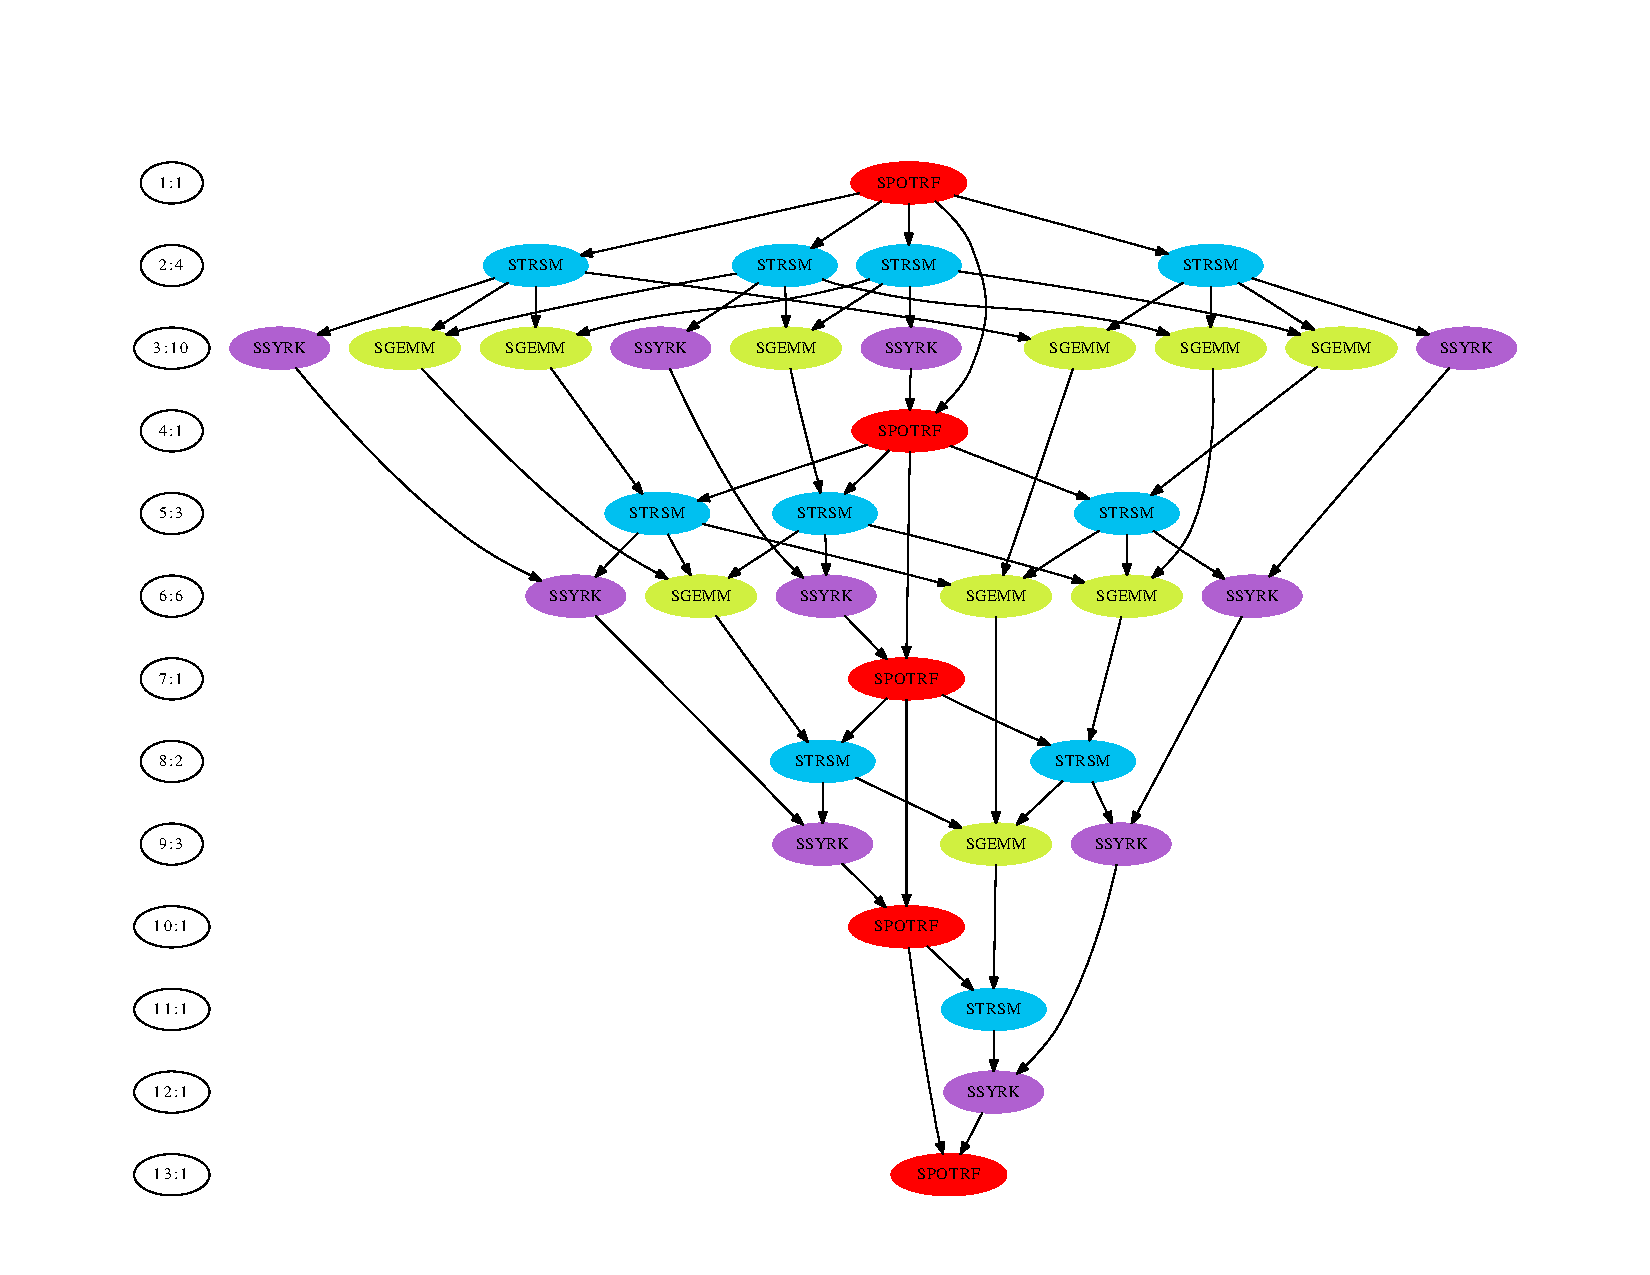
\includegraphics[width=.7\textwidth]{dag-cholesky-5tile.pdf}\\
\caption{DAG of Cholesky for $t=5$. All tasks have unit weight.}
\end{center}
\end{figure}
\end{minipage}
\end{tabular}


\end{frame}


\begin{frame}

%\vspace*{-1cm}
\begin{tabular}{ll}
\begin{minipage}{5cm}
\begin{figure}
\begin{center}
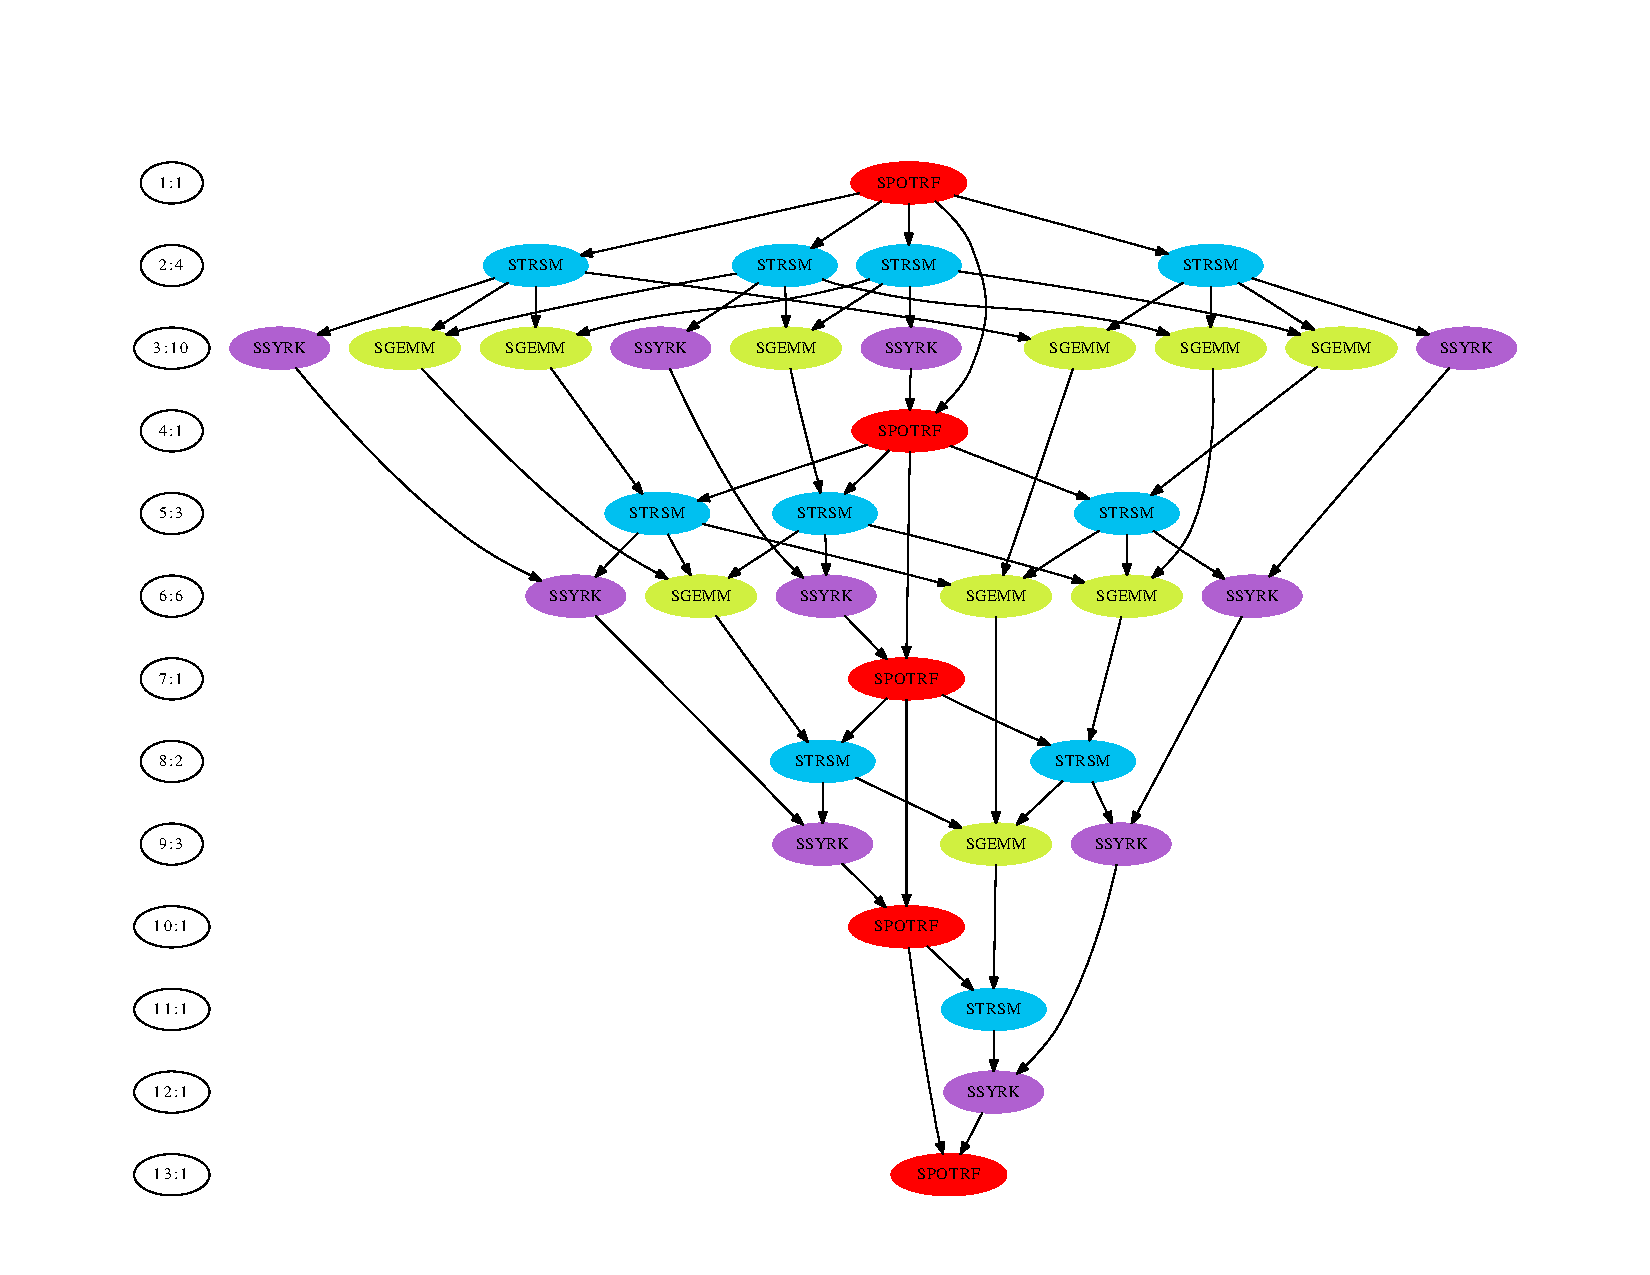
\includegraphics[width=\textwidth]{dag-cholesky-5tile.pdf}\\
\caption{DAG of Cholesky for $t=5$. All tasks have unit weight.}
\end{center}
\end{figure}
\end{minipage}
&
\begin{minipage}{5cm}
\begin{table}
\renewcommand{\arraystretch}{1.6}
\centering
\begin{tabular}{|c|c|}
  \hline
  Type of task & Number of tasks\\
  \hline
  C  & $t$\\
  \hline
  S  & $\frac{t(t-1)}{2}$\\
  \hline
  T  & $\frac{t(t-1)}{2}$ \\
  \hline
  G  & $\frac{t^{3}}{6} - \frac{t^{2}}{2} + \frac{t}{3}$ \\
  \hline
\end{tabular}
\caption {Number of tasks}
\end{table}

\end{minipage}
\end{tabular}


\end{frame}


\begin{frame}

%\vspace*{-1cm}
\begin{tabular}{ll}
\begin{minipage}{5cm}
\begin{figure}
\begin{center}
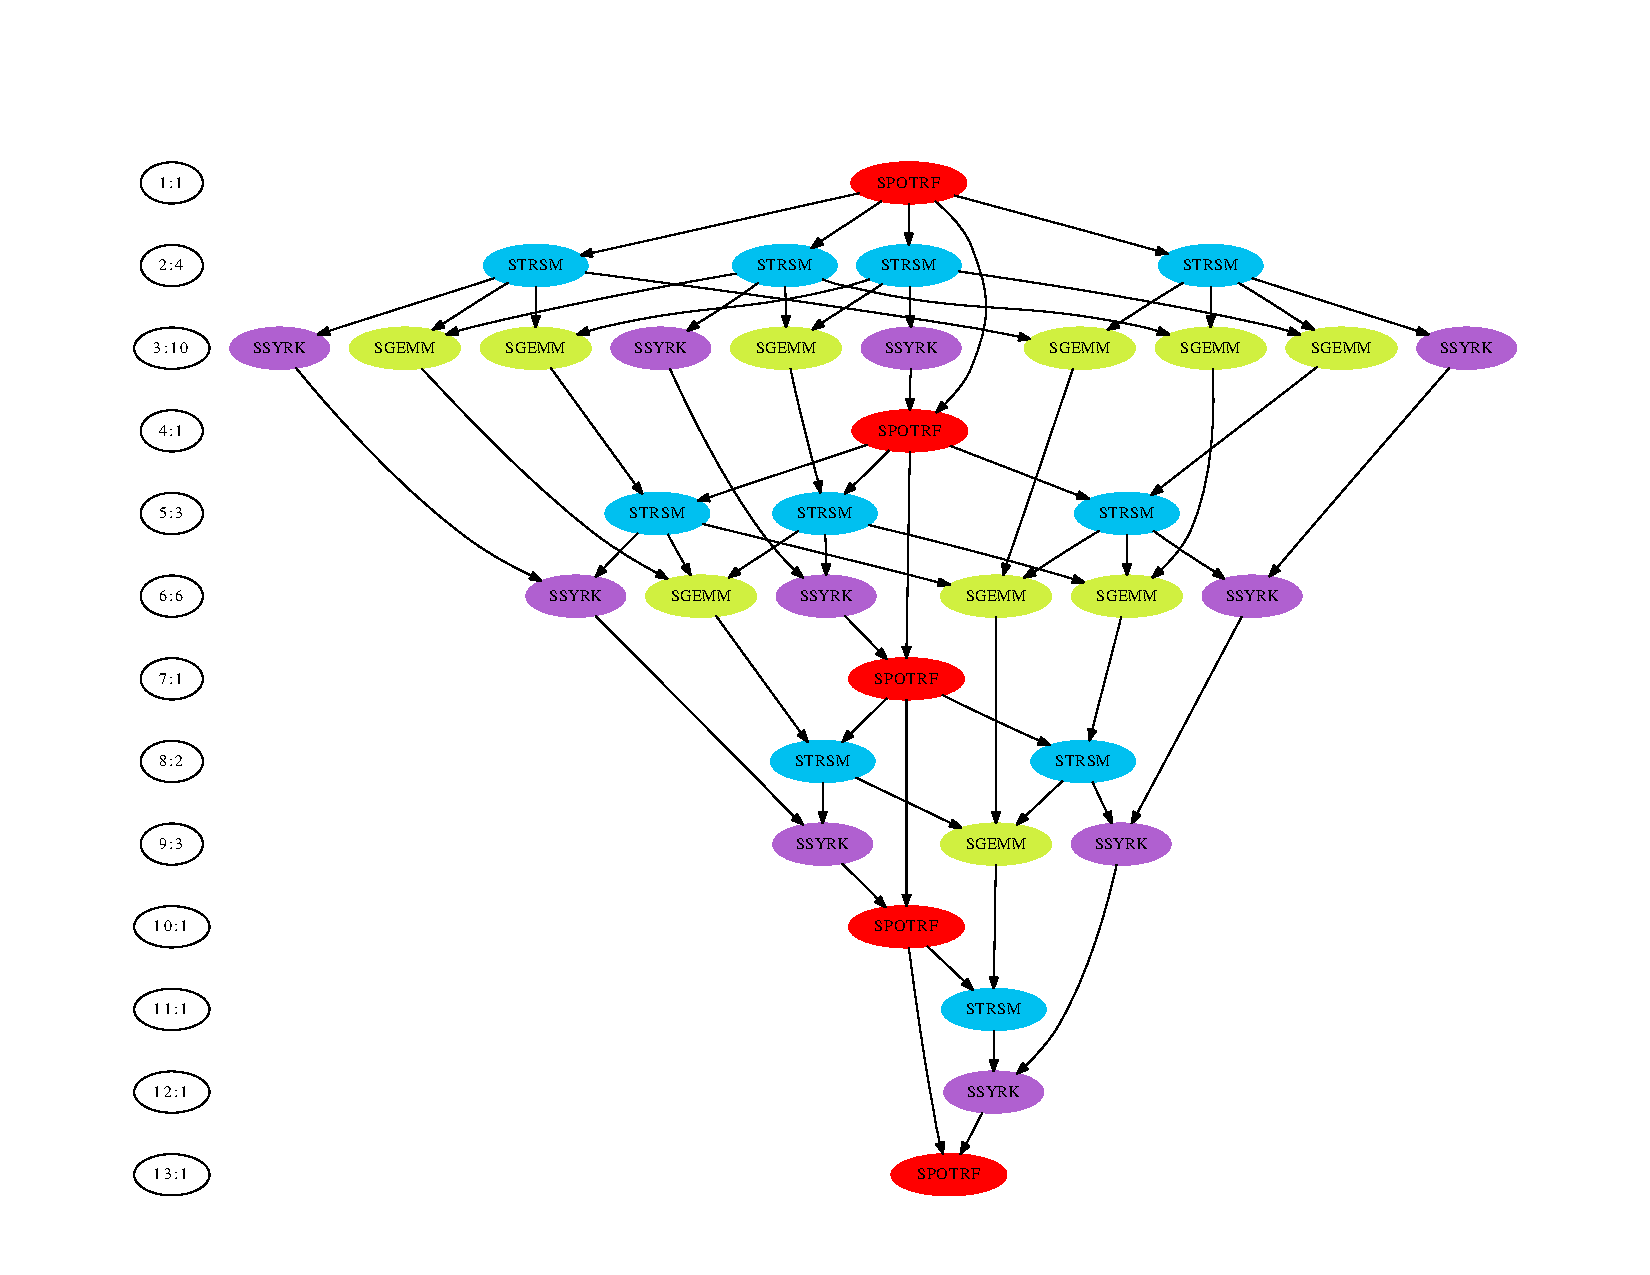
\includegraphics[width=\textwidth]{dag-cholesky-5tile.pdf}\\
\caption{DAG of Cholesky for $t=5$. All tasks have unit weight.}
\end{center}
\end{figure}
\end{minipage}
&
\begin{minipage}{5cm}

\begin{table}[!t]
\tiny
\begin{tabular}{|c|c|c|}
  \hline
  Type of Task & number of Flops & Weight (in $\frac{1}{3}n_{b}^{3}*$Flops) \\
  \hline
  POTRF ($C$) & $\frac{1}{3}n_{b}^{3} + \mathcal{O}(n_{b}^{2})$ & 1 \\
  \hline
  TRSM ($T$)& $n_{b}^{3}$ & 3\\
    \hline
  SYRK ($S$)& $n_{b}^{3} + \mathcal{O}(n_{b}^{2})$ & 3 \\
    \hline
  GEMM ($G$)& $2n_{b}^{3} + \mathcal{O}(n_{b}^{2})$ & 6 \\
  \hline
\end{tabular}
\caption {Task weights for the Cholesky factorization}
\end{table}

\end{minipage}
\end{tabular}


\end{frame}

\begin{frame}

\begin{figure}
\begin{center}
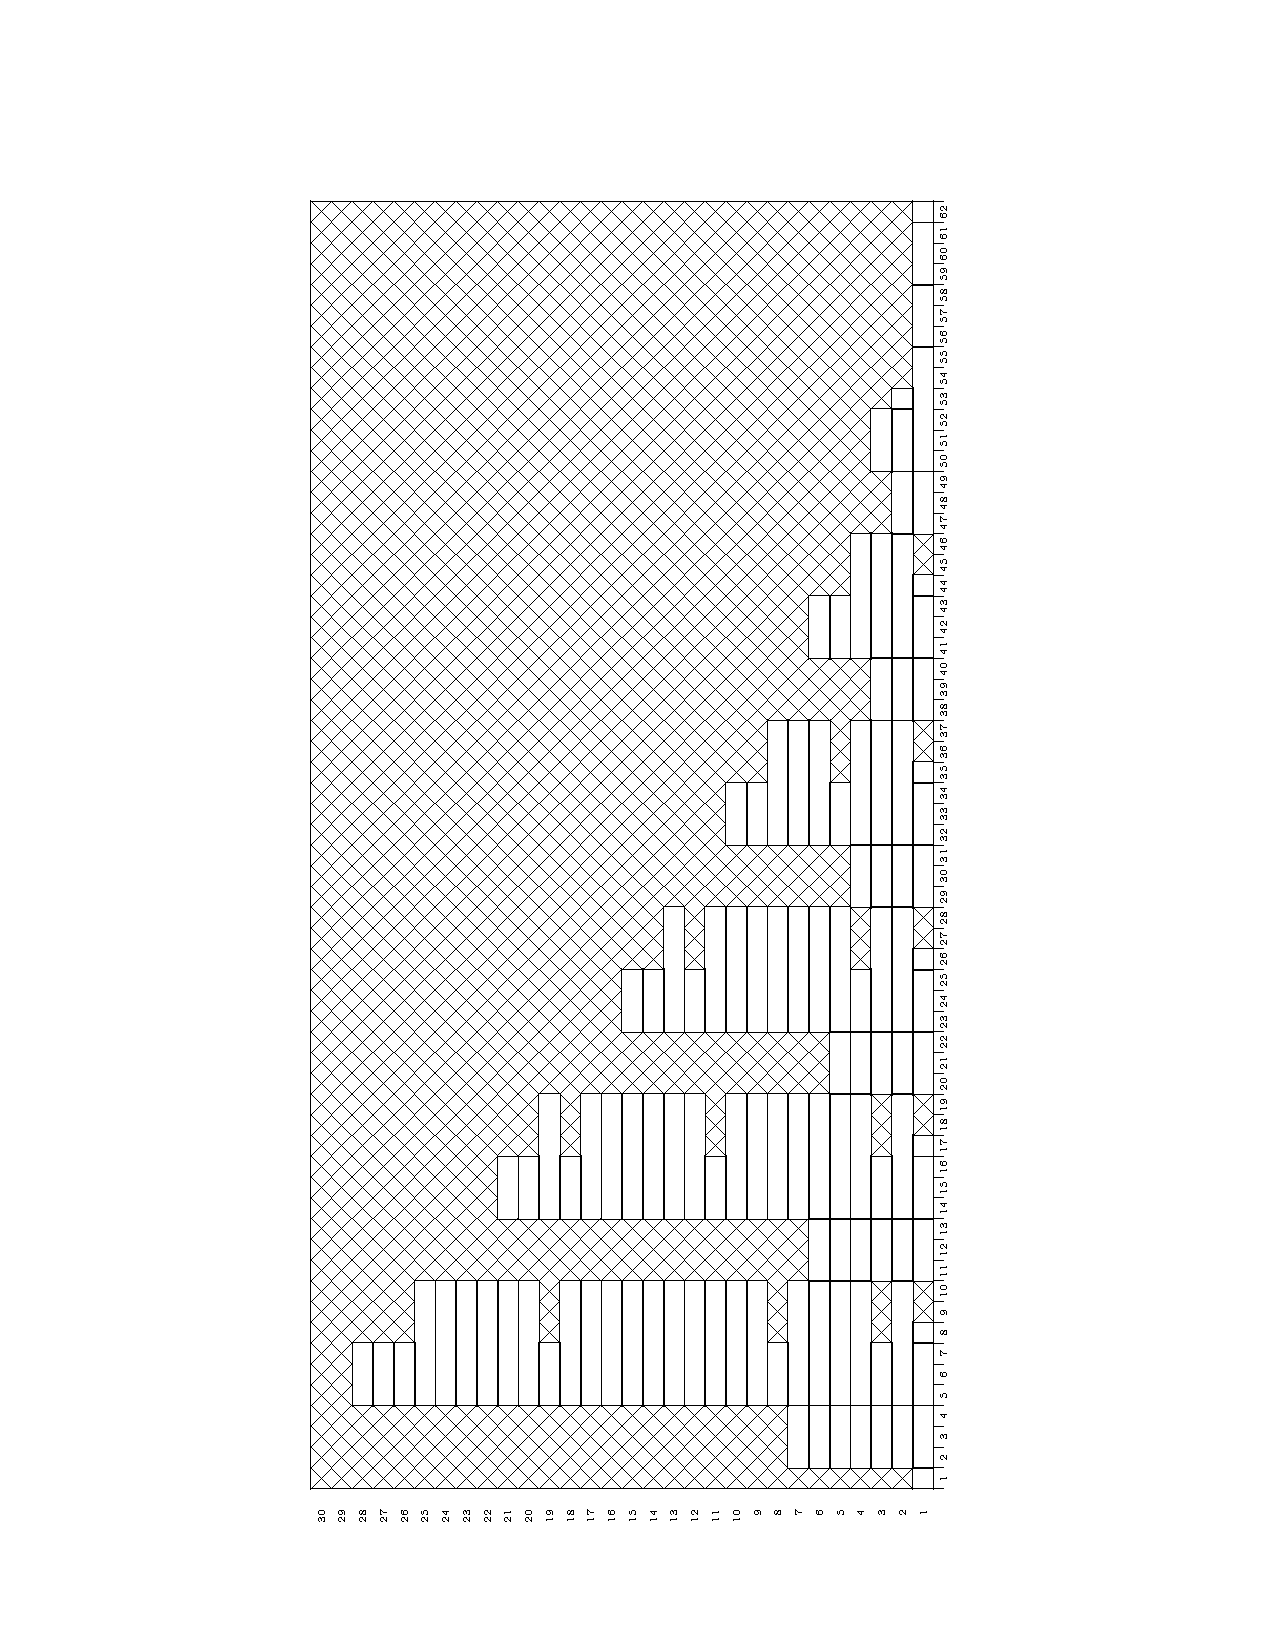
\includegraphics[width=.5\textwidth,angle=270]{./fig/t8_p30_fwd.pdf}
\caption{Schedule of Cholesky for $t=8$ using unbounded number of resources.}
\end{center}
\end{figure}


\end{frame}






\begin{frame}

%\vspace*{-1cm}
\begin{tabular}{ll}
\begin{minipage}{11cm}
\begin{figure}
\begin{center}
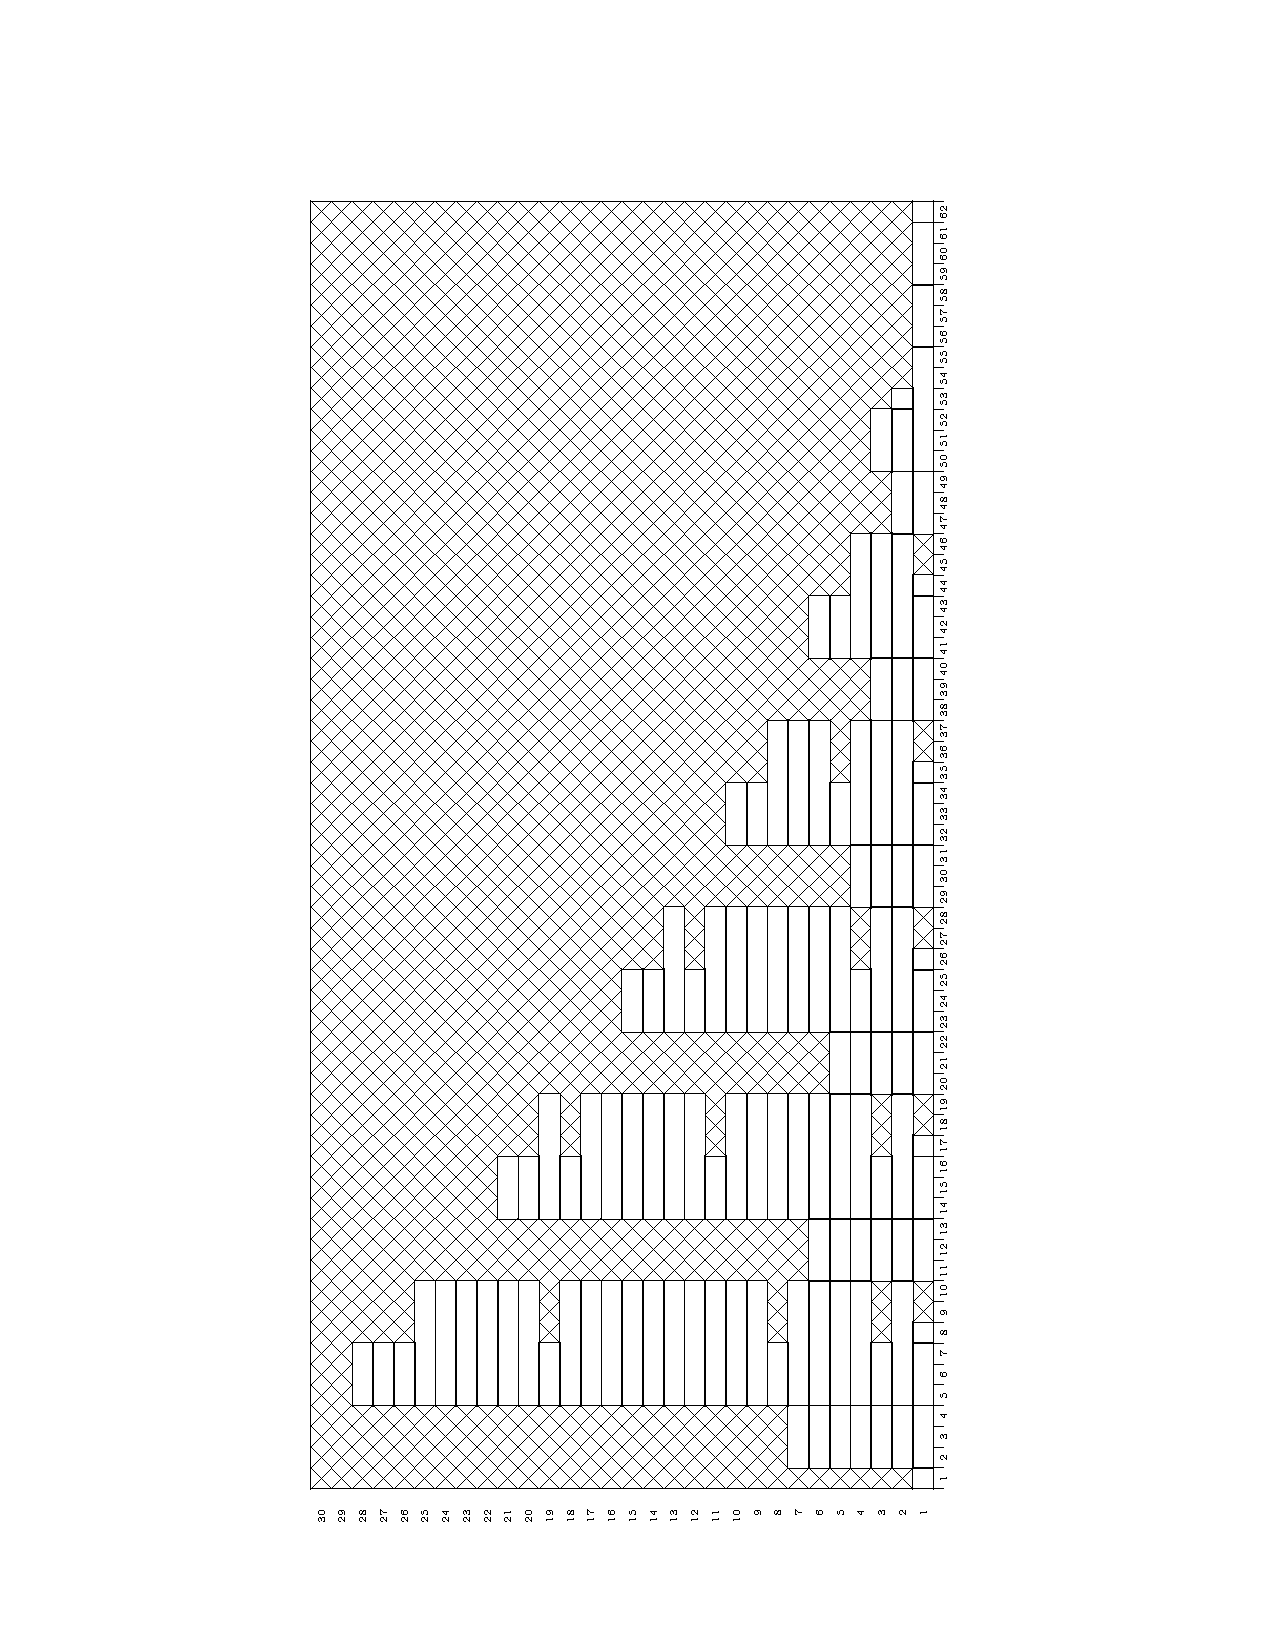
\includegraphics[width=.20\textwidth,angle=270]{./fig/t8_p30_fwd.pdf}
\caption{
\footnotesize
Schedule of Cholesky for $t=8$ using unbounded number of resources.}
\end{center}
\end{figure}
\end{minipage}
\\
\begin{minipage}{11cm}
\footnotesize
\begin{tabular}{ll}

\underline{\textsc{Work:}} Weight of all the tasks is $t^3.$& ( 512, for $t=8$ )\\
\\
\underline{\textsc{Length:}} (or execution time)
or (weighted) critical path length is $9t-10.$&( 62, for $t=8$  )\\
\\
\underline{\textsc{Height:}} number of resources needed for ASAP schedule is $\frac{1}{2}t^2-\frac{1}{2}t.$ & ( 28, for $t=8$  )\\
\\
\underline{\textsc{Idle:}} (for ASAP) 
$(9t-10)(\frac{1}{2}t^2-\frac{1}{2}t) - t^3$ is
$\approx \frac{7}{2}t^3.$ & ( 1,224, for $t=8$ )\\
\\
{\color{CUGold} ASAP:} $\frac{2}{9}\approx0.222\%$ work, $\frac{7}{9}\approx0.778\%$ idle & 29\% work\\& 71\% idle \\

\end{tabular}


\end{minipage}
\end{tabular}


\end{frame}



\begin{frame}
ASAP schedule $t=8$ and $p=\infty$~~~~~~~~~~
ALAP schedule $t=8$ and $p=\infty$\\
  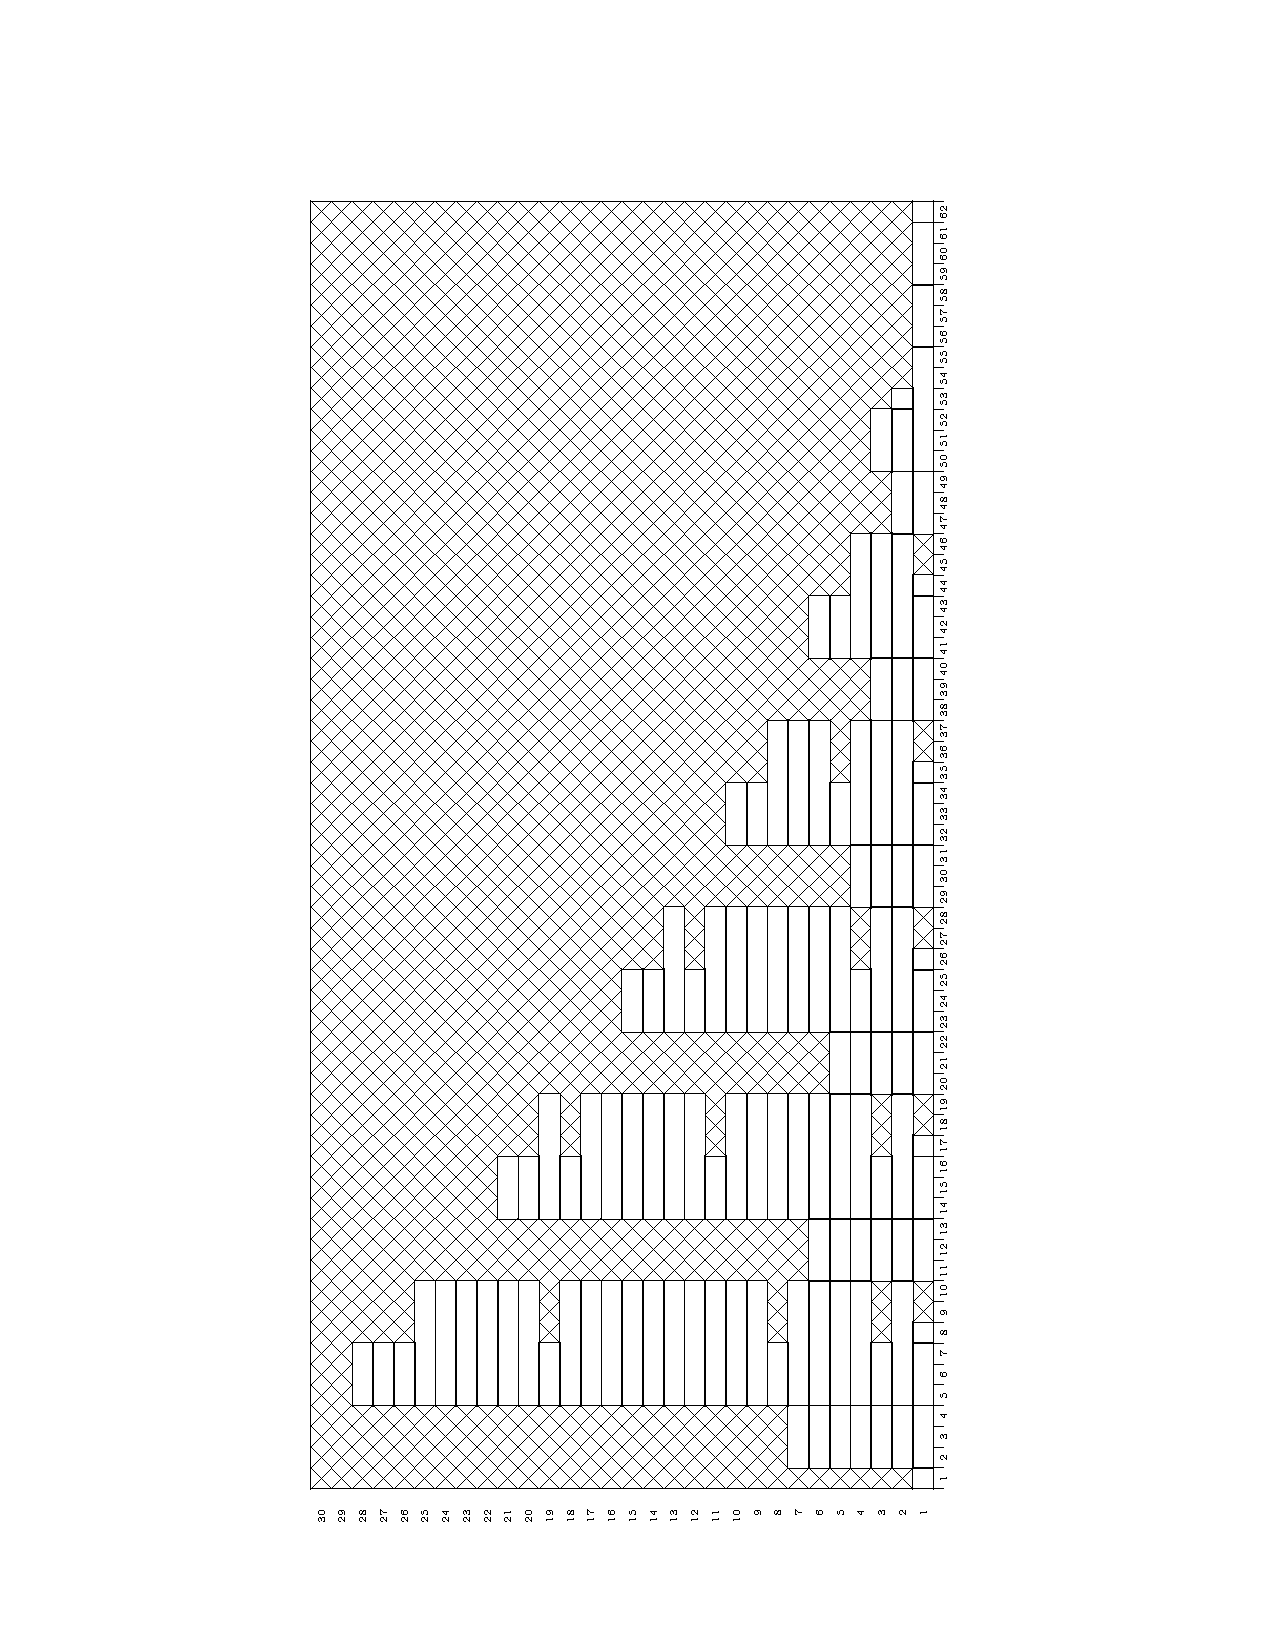
\includegraphics[width=.25\textwidth,angle=270]{./fig/t8_p30_fwd.pdf}
  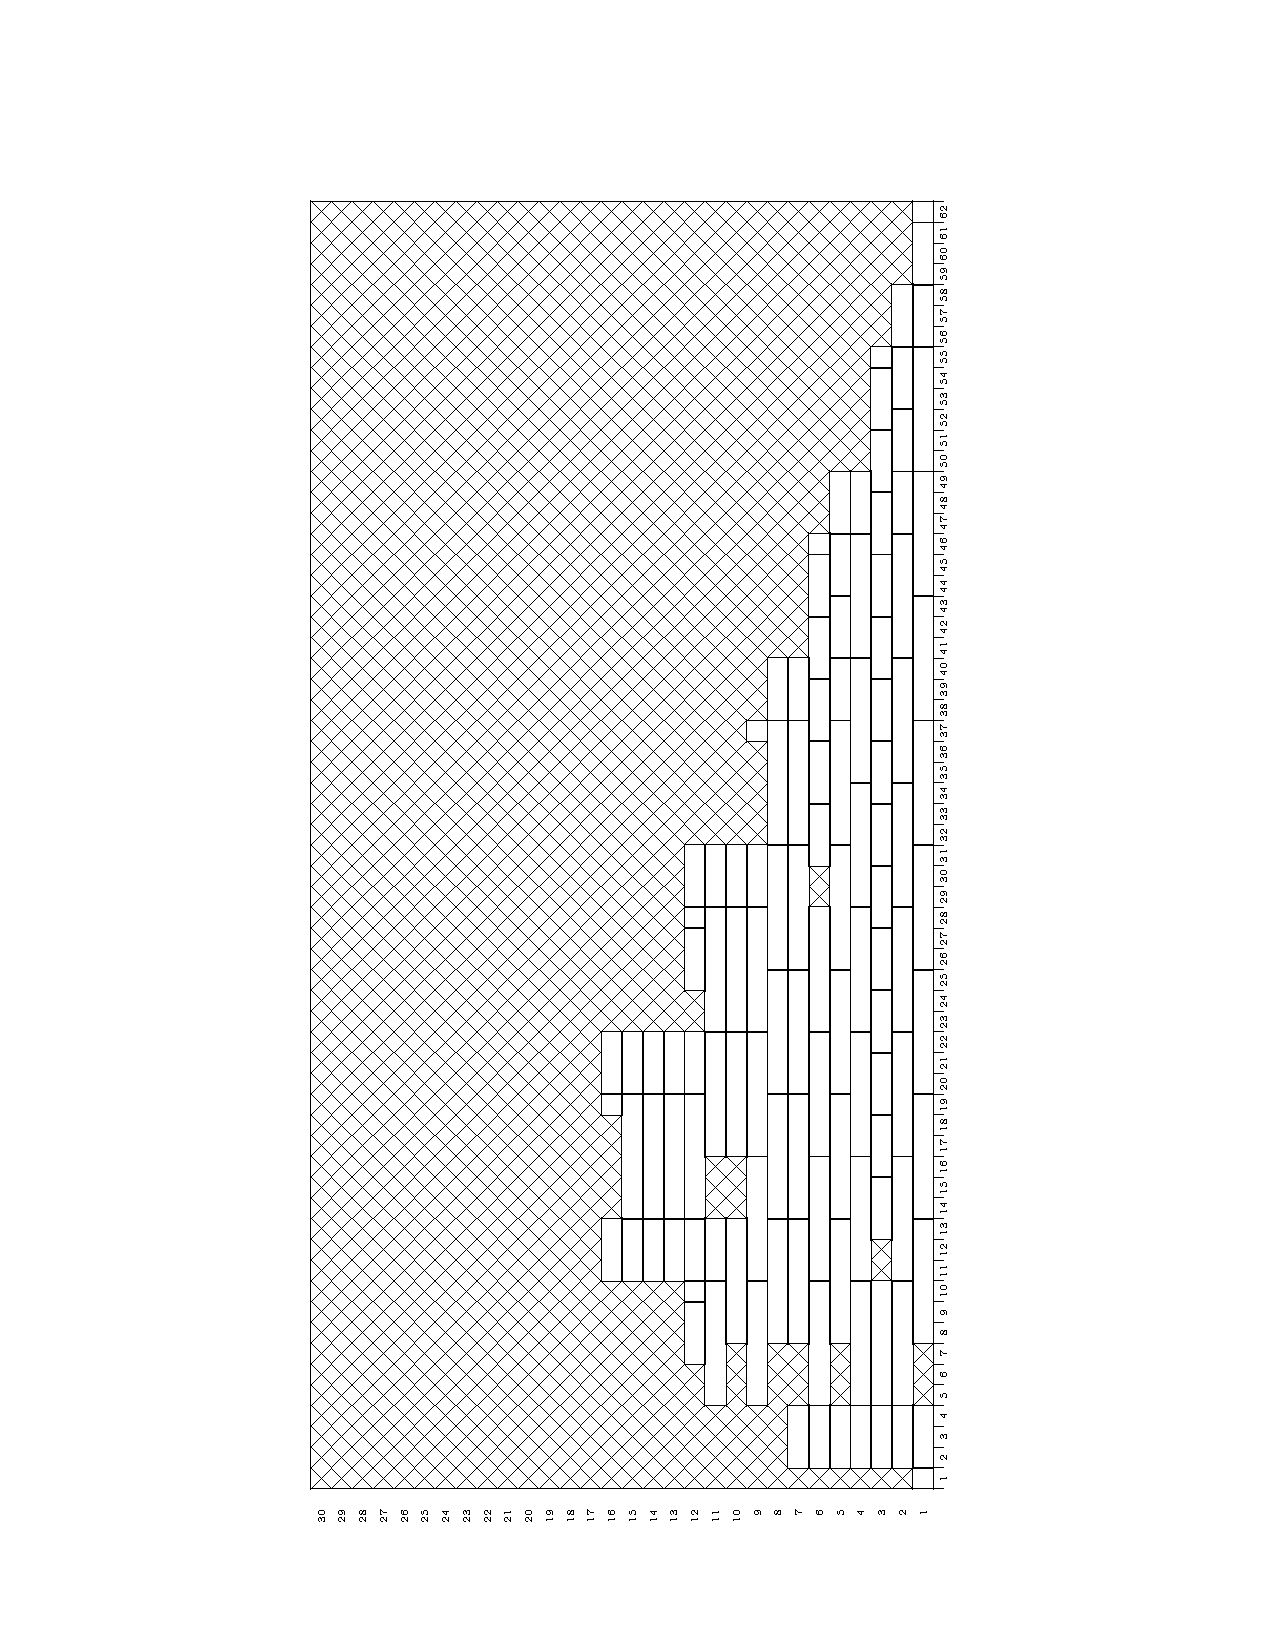
\includegraphics[width=.25\textwidth,angle=270]{./fig/t8_p30_bwd.pdf}\\
Length of the critical path: $62$

\end{frame}








\begin{frame}

\begin{figure}[!t]
\centering
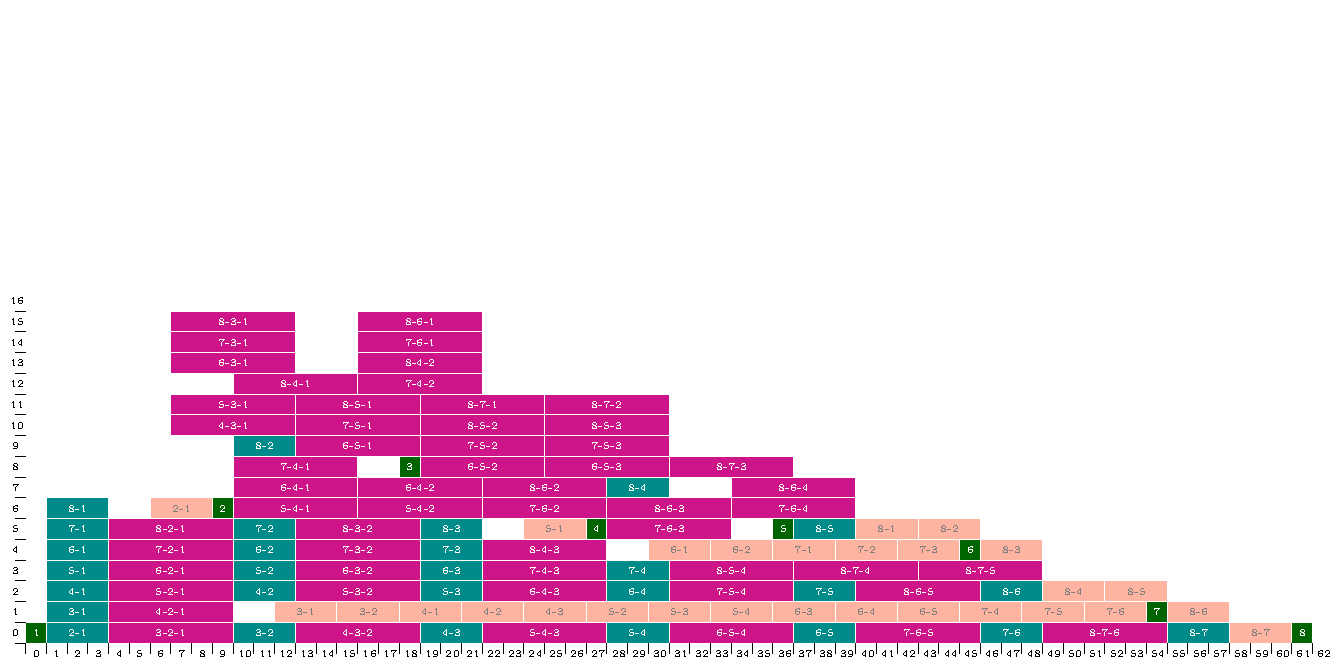
\includegraphics[width=4.7in]{fig/ALAP_08x08.pdf}
\caption{ALAP schedule on $8 \times 8$ tiles. Dark green POTRF, light green for
TRSM, salmon for SYRK, and magenta for GEMM.  Time is in the x-axis. Execution
time is the critical path length: $9t-10 = 62$. Number of required processing
units for the schedule is 16.
}
\end{figure}

\end{frame}



\begin{frame}

%\vspace*{-1cm}
\begin{tabular}{ll}
\begin{minipage}{11cm}
\begin{figure}
\begin{center}
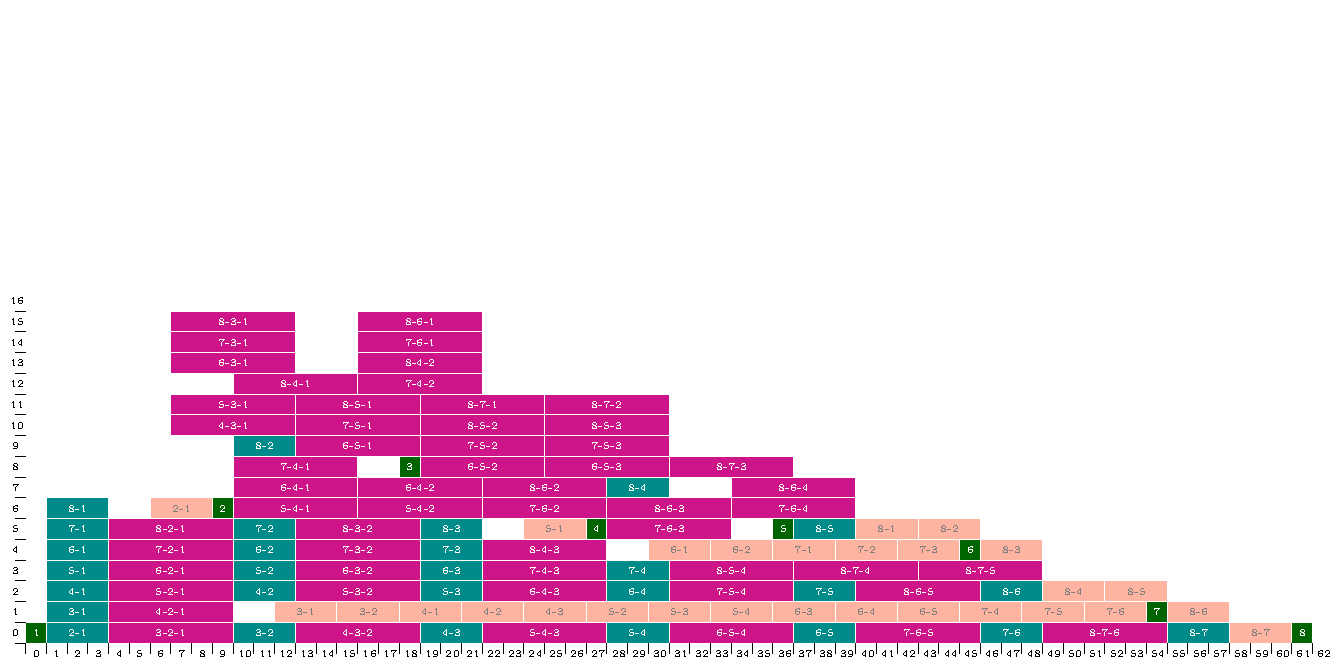
\includegraphics[width=3in]{fig/ALAP_08x08.pdf}
\caption{
\footnotesize
Schedule of Cholesky for $t=8$ using unbounded number of resources.}
\end{center}
\end{figure}
\end{minipage}
\\
\begin{minipage}{11cm}
\footnotesize
\begin{tabular}{ll}

\underline{\textsc{Work:}} Weight of all the tasks is $t^3.$& ( 512, for $t=8$ )\\
\\
\underline{\textsc{Length:}} (or execution time)
or (weighted) critical path length is $9t-10.$&( 62, for $t=8$  )\\
\\
\underline{\textsc{Height:}} number of resources needed for ALAP schedule is $\approx \frac{1}{4}t^2+\frac{1}{8}t.$ & ( 16, for $t=8$  )\\
\\
\underline{\textsc{Idle:}} (for ALAP) 
$(9t-10)(\frac{1}{4}t^2+\frac{1}{8}t) - t^3$ is
$\approx \frac{5}{4}t^3.$ & ( 480, for $t=8$ )\\
\\
{\color{CUGold} ALAP:} $\frac{4}{9}\approx0.444\%$ work, $\frac{5}{9}\approx0.556\%$ idle & 52\% work\\& 48\% idle\\

\end{tabular}


\end{minipage}
\end{tabular}


\end{frame}





\begin{frame}
ASAP schedule $t=8$ and $p=\infty$\\

  {\begin{minipage}{.25\textwidth}\vspace*{-2.8cm}
  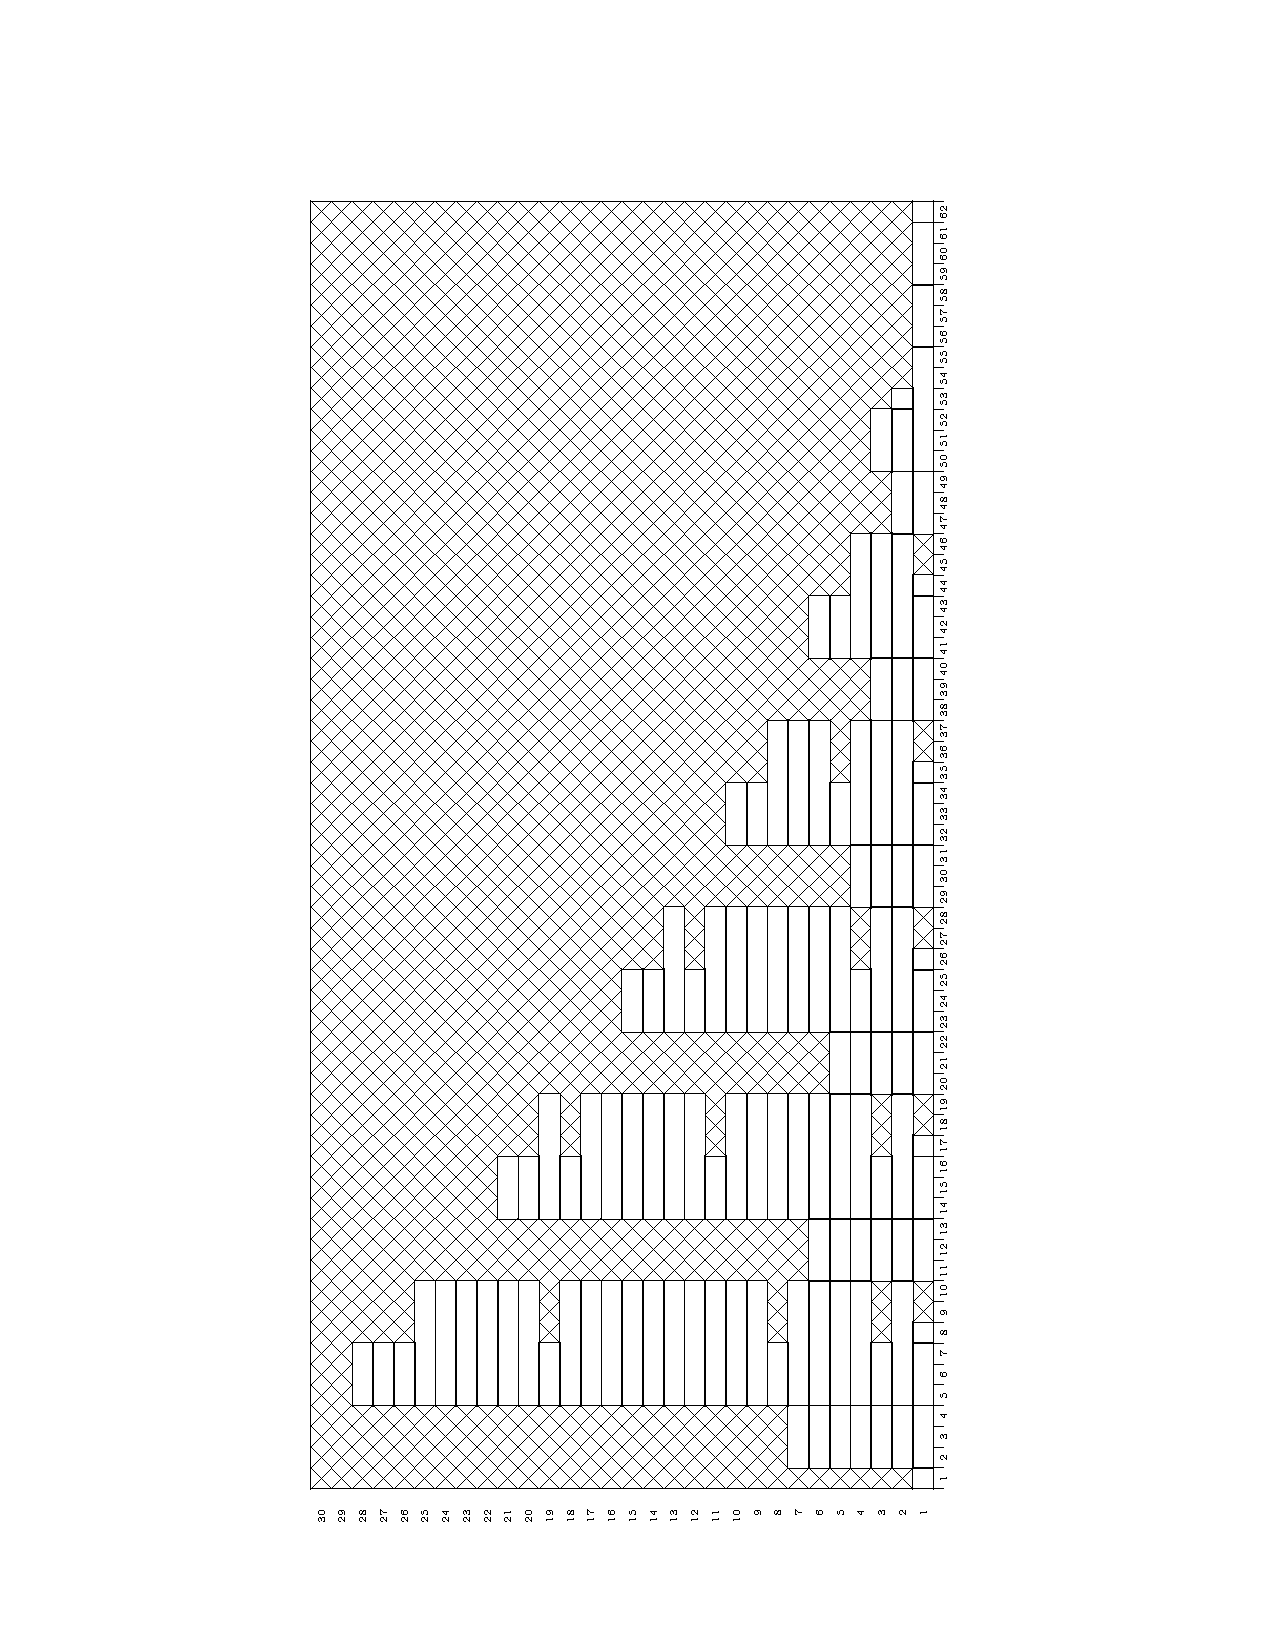
\includegraphics[width=\textwidth,angle=270]{./fig/t8_p30_fwd.pdf}\end{minipage}}
  ~~~~~~~~~~~~~~~~~~~~~~~~~~~~~~~~~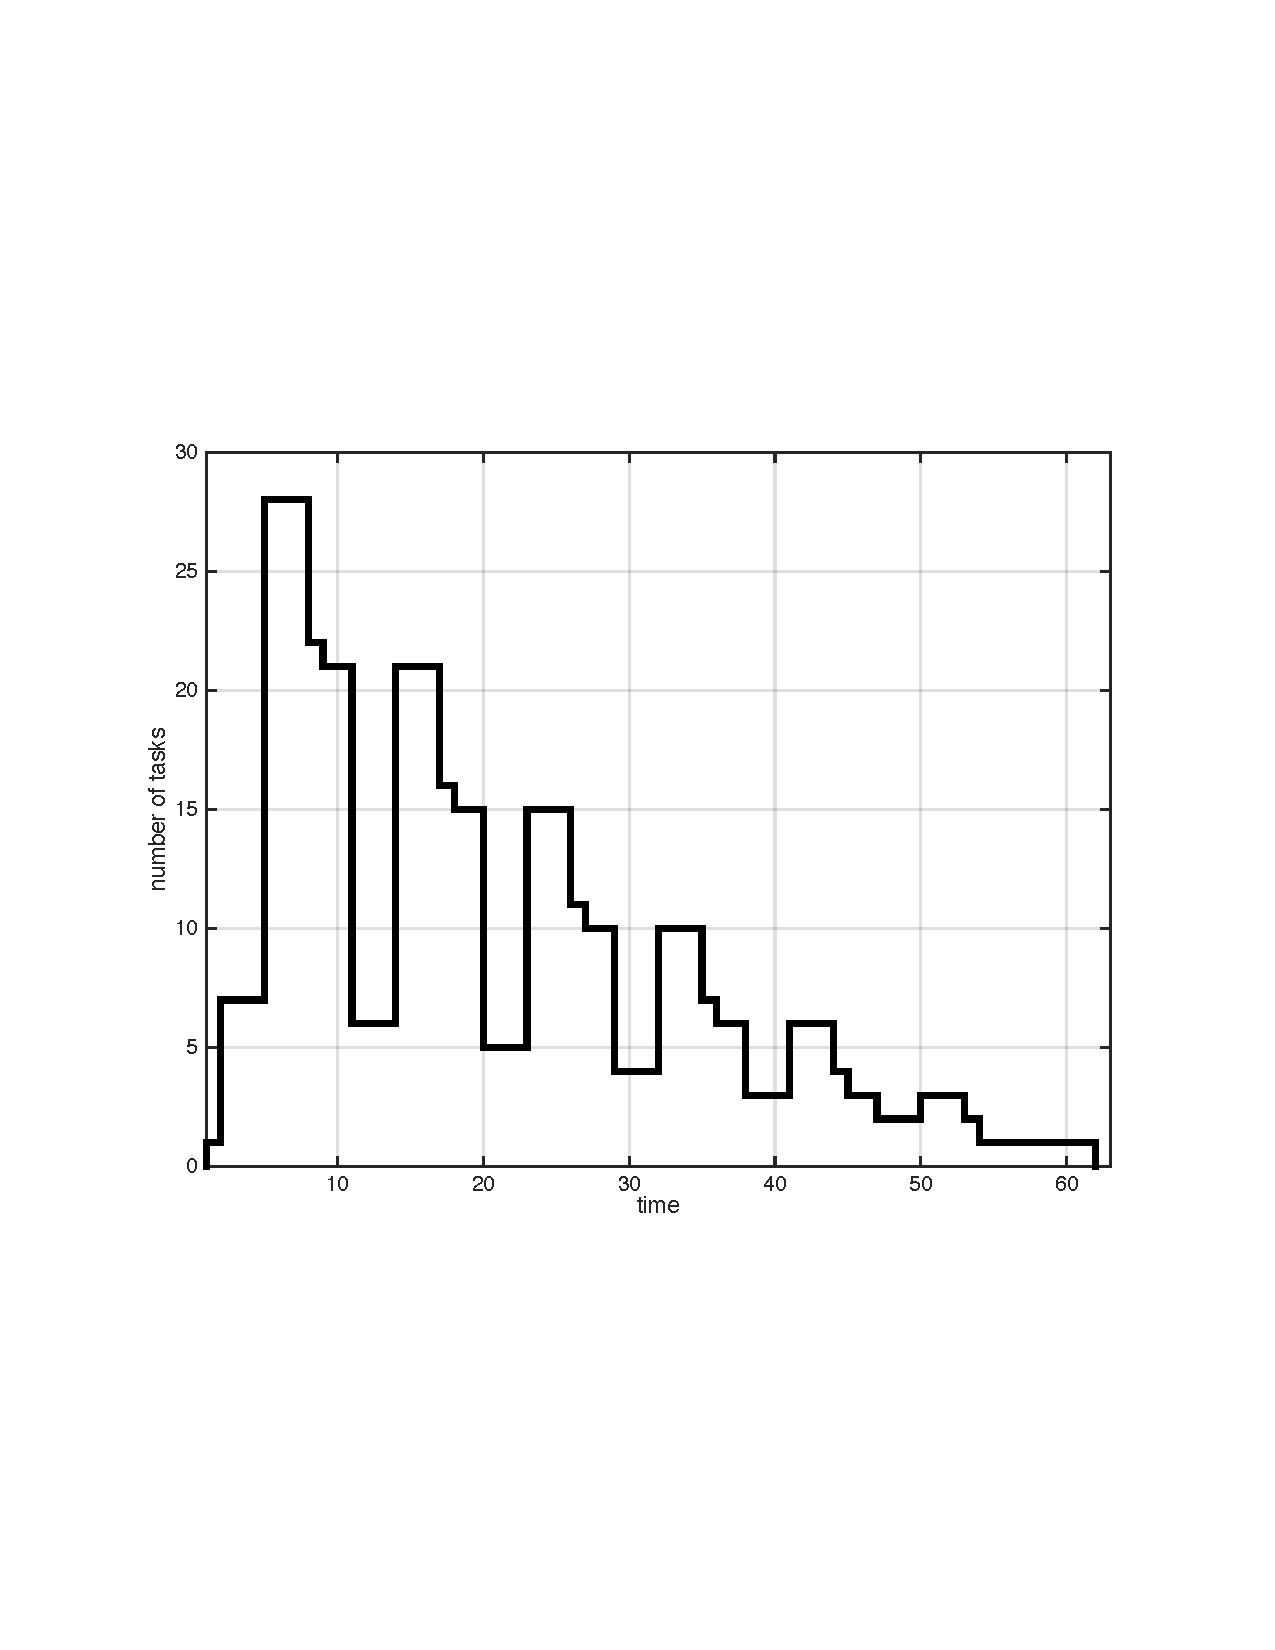
\includegraphics[width=.35\textwidth]{matlab_files/qqq_t8__asap.pdf}\\

Length of the critical path: $62$

\end{frame}




\begin{frame}
ALAP schedule $t=8$ and $p=\infty$\\

  {\begin{minipage}{.25\textwidth}\vspace*{-2.8cm}
  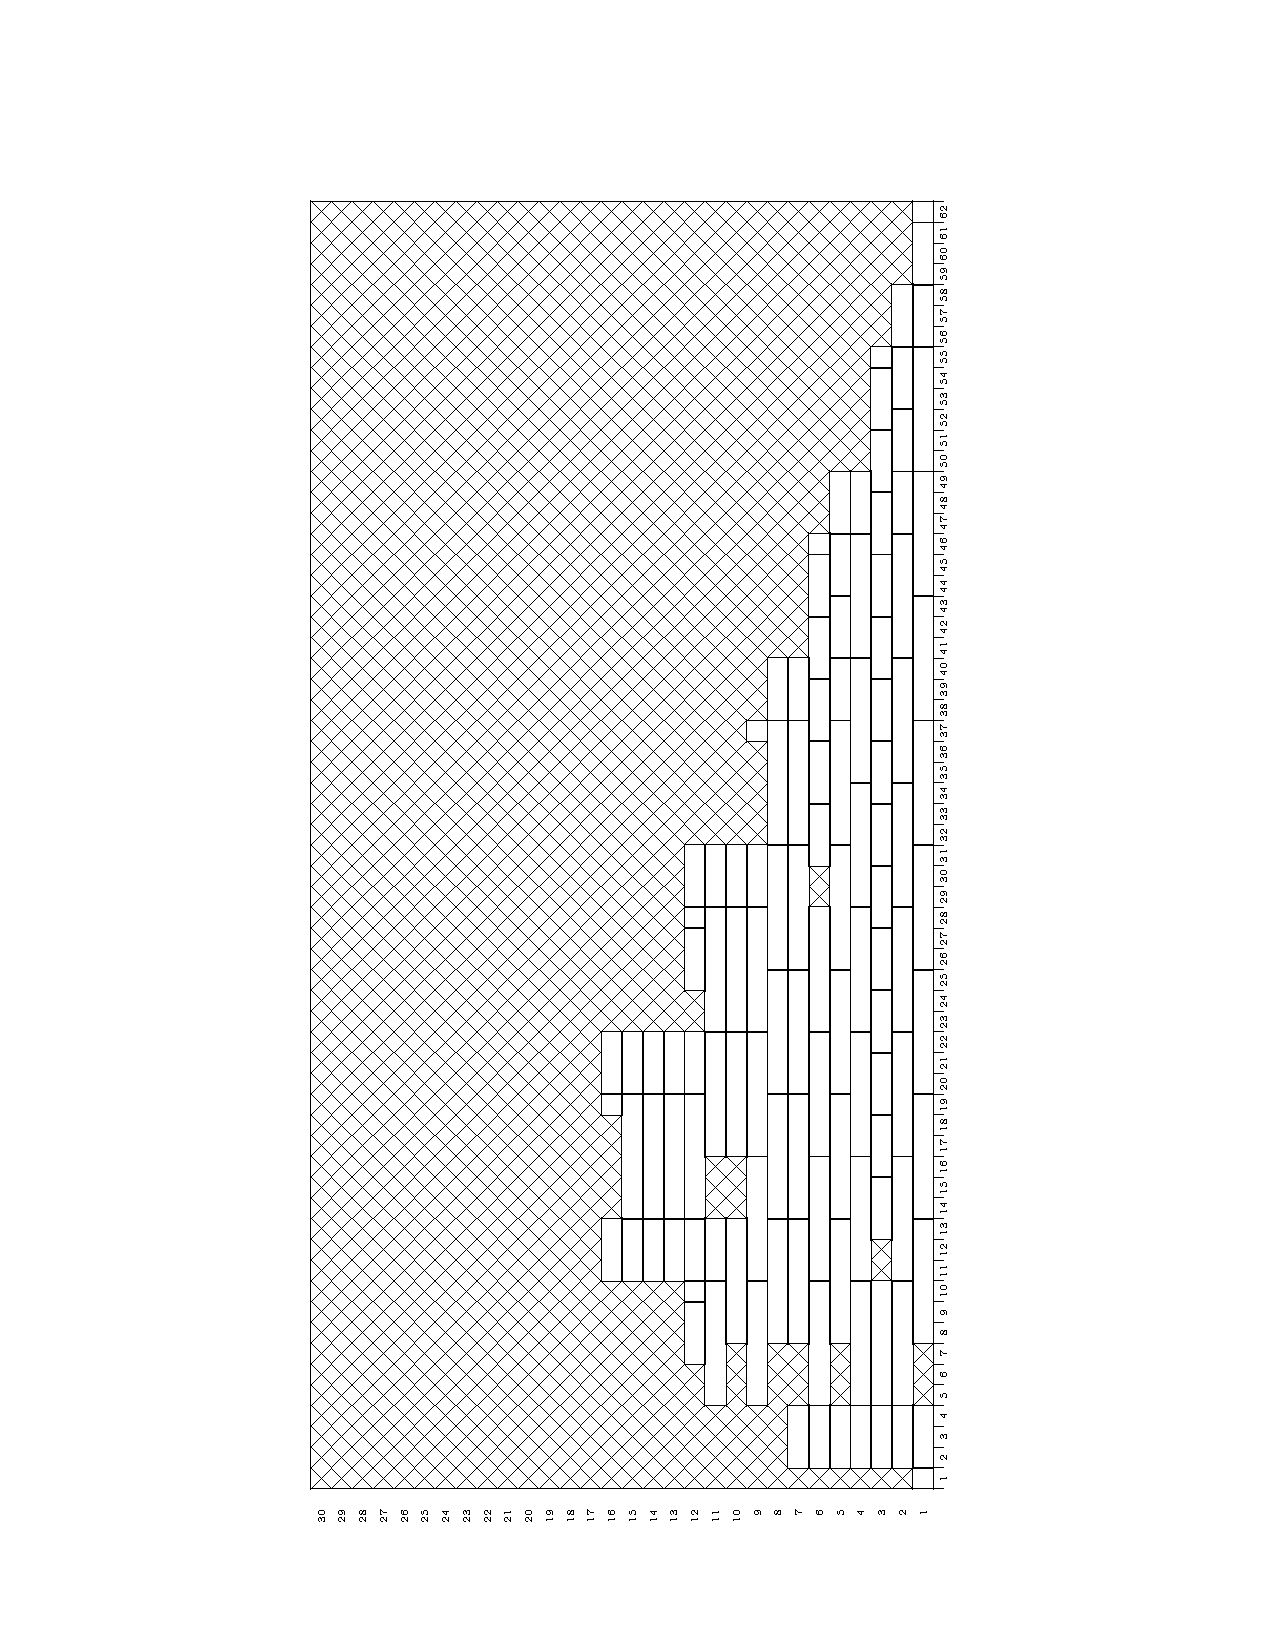
\includegraphics[width=\textwidth,angle=270]{./fig/t8_p30_bwd.pdf}\end{minipage}}
  ~~~~~~~~~~~~~~~~~~~~~~~~~~~~~~~~~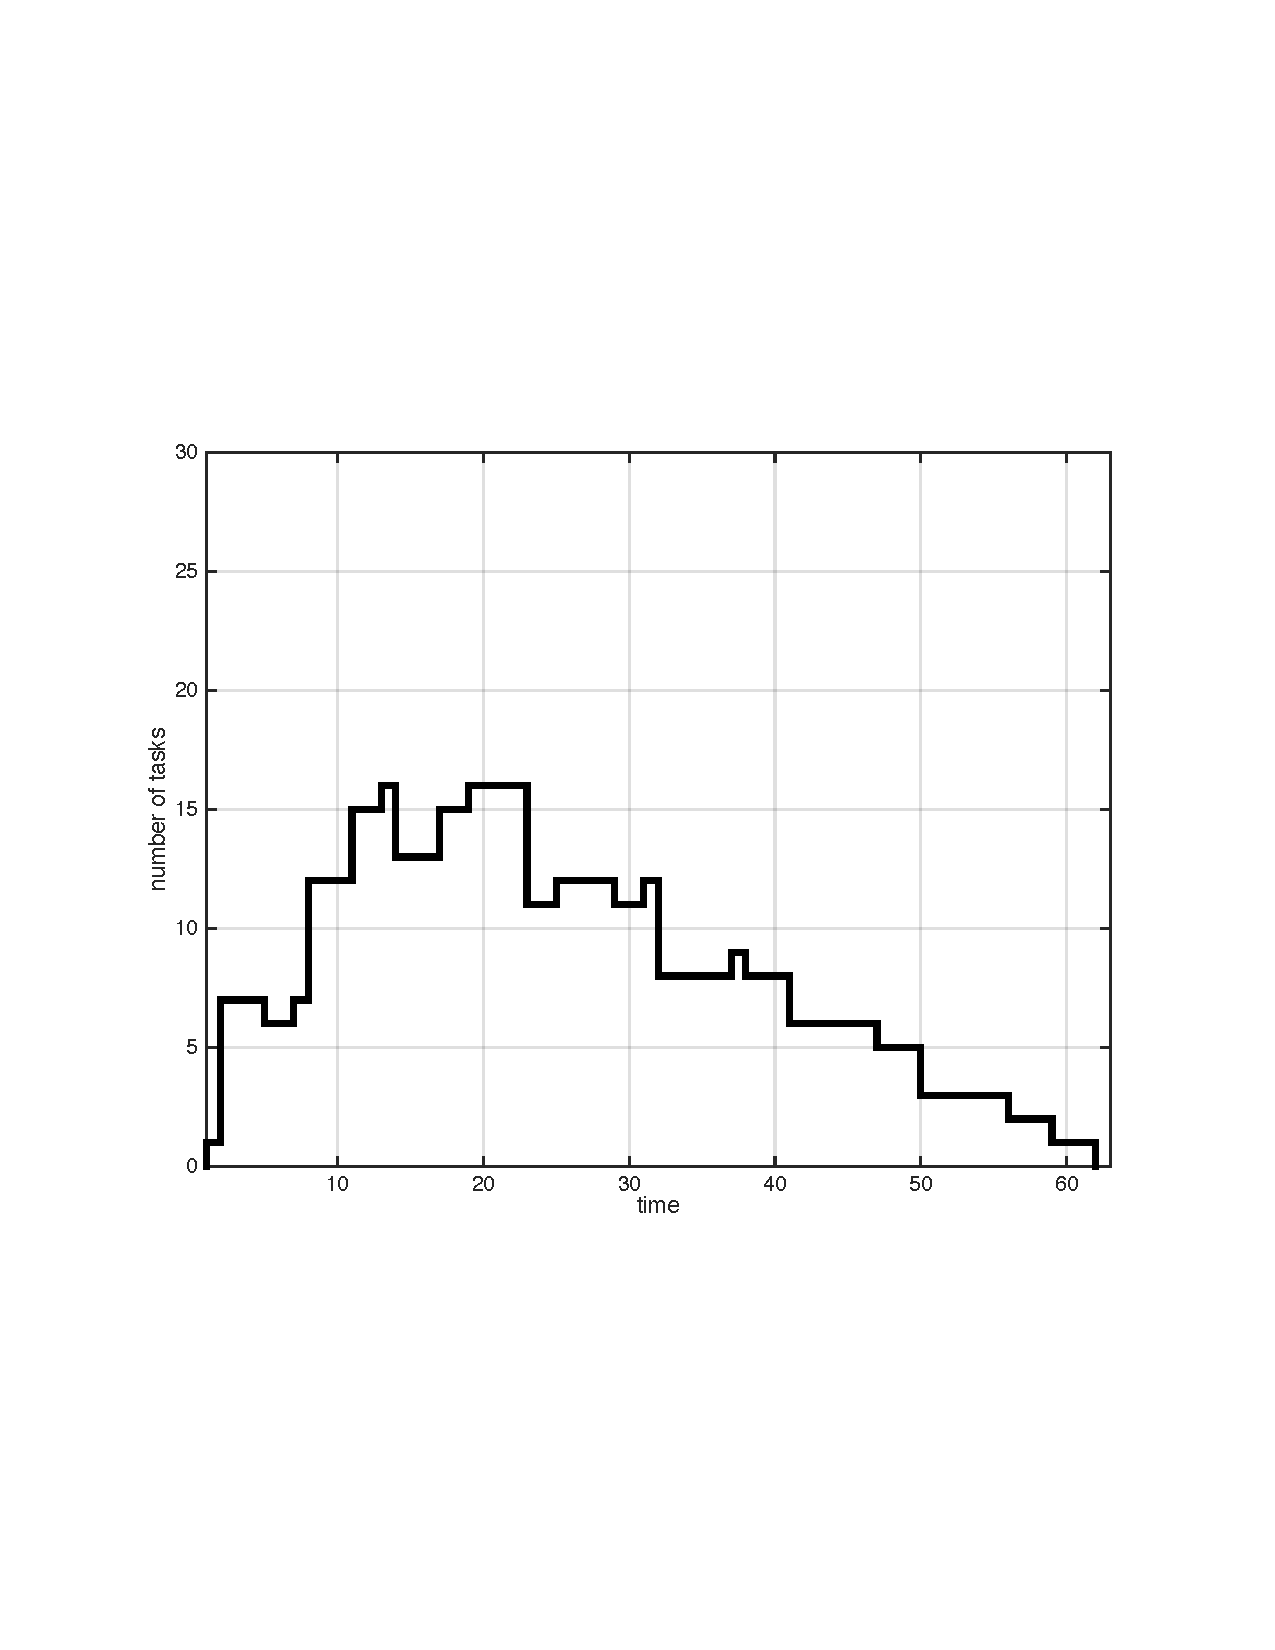
\includegraphics[width=.45\textwidth]{matlab_files/qqq_t8_v2.pdf}\\

Length of the critical path: $62$

\end{frame}



\begin{frame}
\tiny
\begin{table}
\renewcommand{\arraystretch}{1.6}
\caption {The heights of the ALAP schedule}
\centering
\begin{tabular}{|c|}
\hline
\begin{minipage}{7cm}
$M_{X,K}$ is the number of
tasks of type X being executed at time $\tau - K$ in an ALAP schedule with
sufficiently many processing units.
\begin{eqnarray}
\nonumber
M_{C,K} & = &
\left\{\begin{array}{cl}
1&\textmd{ if } K = 9\ell +8,\\
0&\textmd{ else.}
\end{array}\right.\\
\nonumber
M_{T,K} & = &
\left\{\begin{array}{cl}
\ell+1&\textmd{ if } 9\ell + 5 \leq K \leq  9\ell + 7\\
0&\textmd{ else.}
\end{array}\right.\\
\nonumber
M_{S,K} & = &
\left\{\begin{array}{cl}

i_{max}  %verifier le 7/12, vrai experimentalement mais bon
- i_{min} +2&\textmd{if } 2\leq K \leq 3t -2\\
\\
i_{max}  %verifier le 7/12, vrai experimentalement mais bon
- i_{min} +1 &\textmd{otherwise}
\end{array}\right.\\
\nonumber
%%%%%%
M_{G,K} & = &
\sum_{j = j_{min}+1}^{j_{max}}
\left( t - j \right)
\end{eqnarray}
where $i_{max} = \min\left(t, \lfloor \frac{3t}{2} - \frac{K}{6} - \frac{7}{12}
\rfloor \right)$ and $i_{min} = \lceil t - \frac{K}{9}\rceil$ denote the two
extremal S-floors executed at time $\tau-K$, and $j_{max} = \min\left(t-1,
\lfloor 3t - \frac{K}{3} - \frac{8}{3}\rfloor \right)$, $j_{min} = \lceil t -
\frac{K}{9} - \frac{2}{9}\rceil$ are as defined above.
\end{minipage}\\
\hline
\end{tabular}
\end{table}


\end{frame}

\begin{frame}

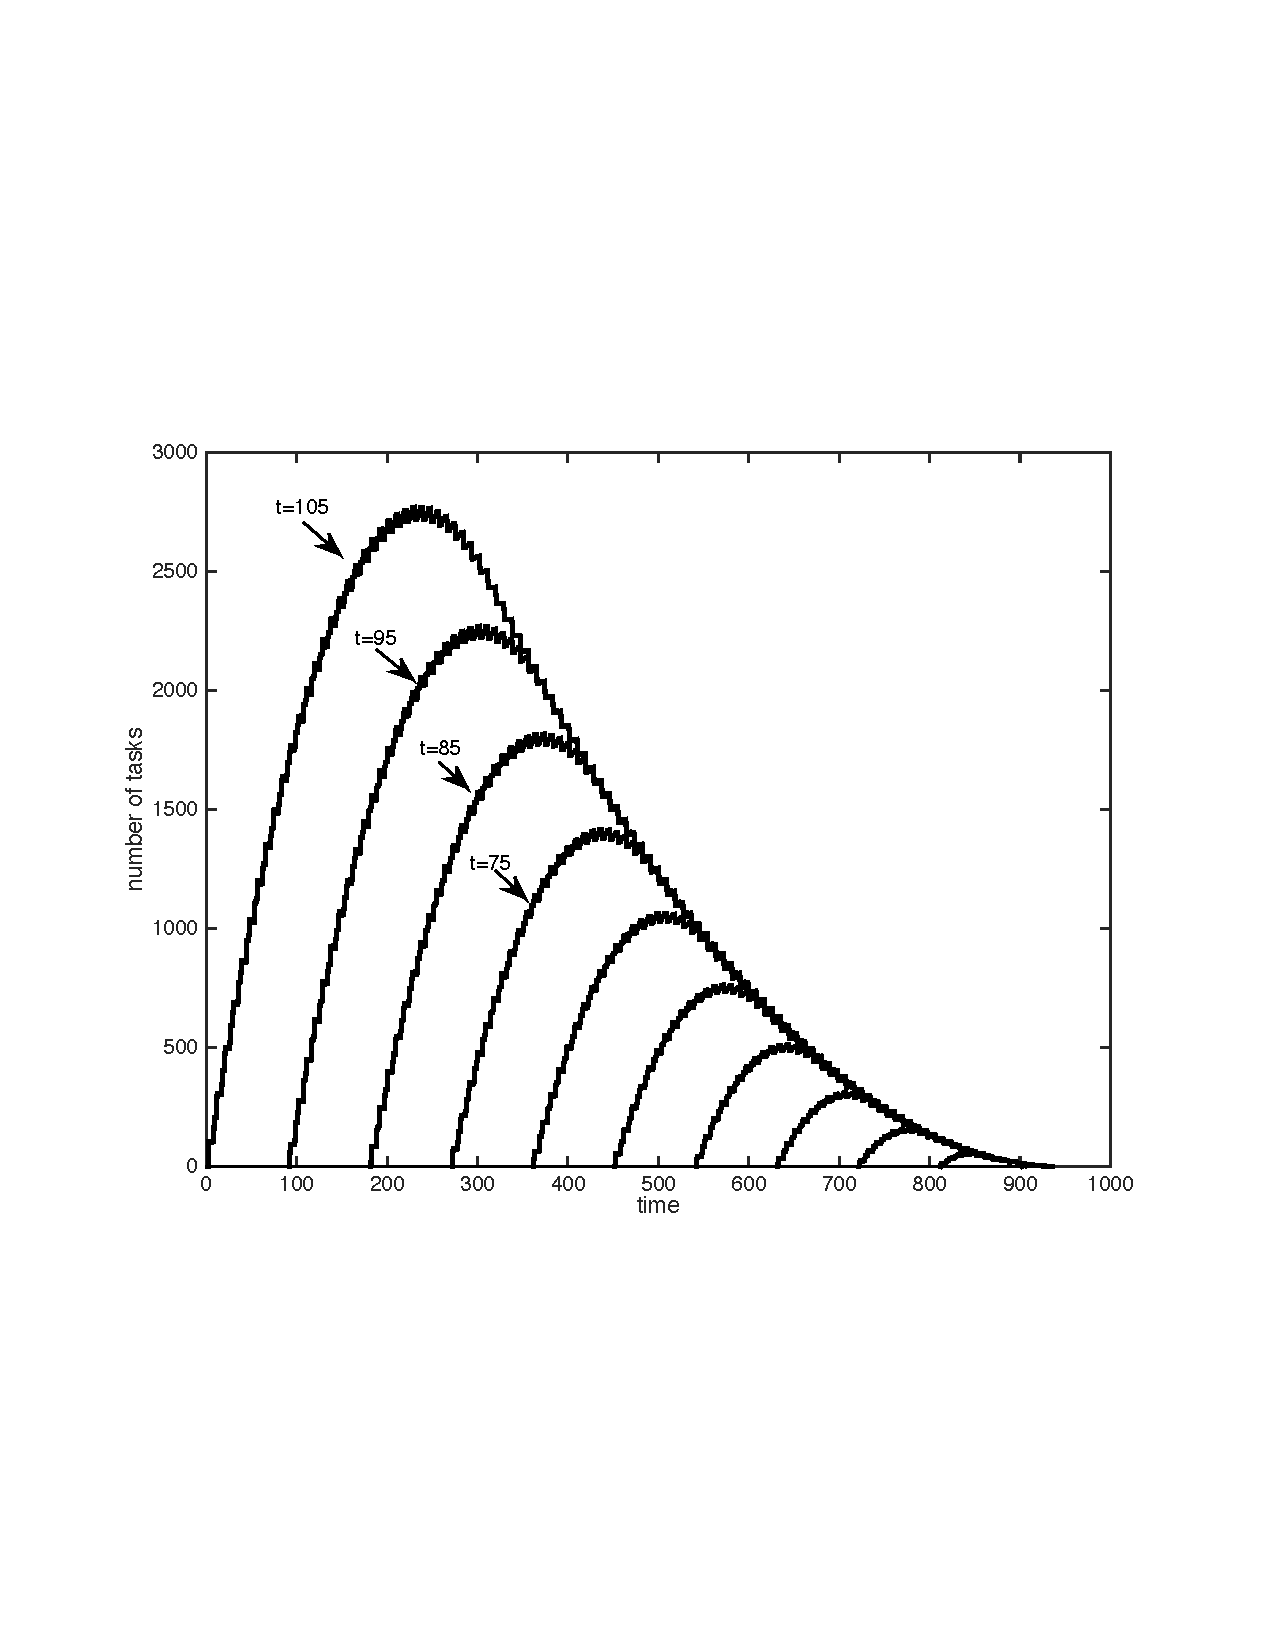
\includegraphics[width=.80\textwidth]{matlab_files/escargots_100_by_10__v2.pdf}\\

\end{frame}

\begin{frame}

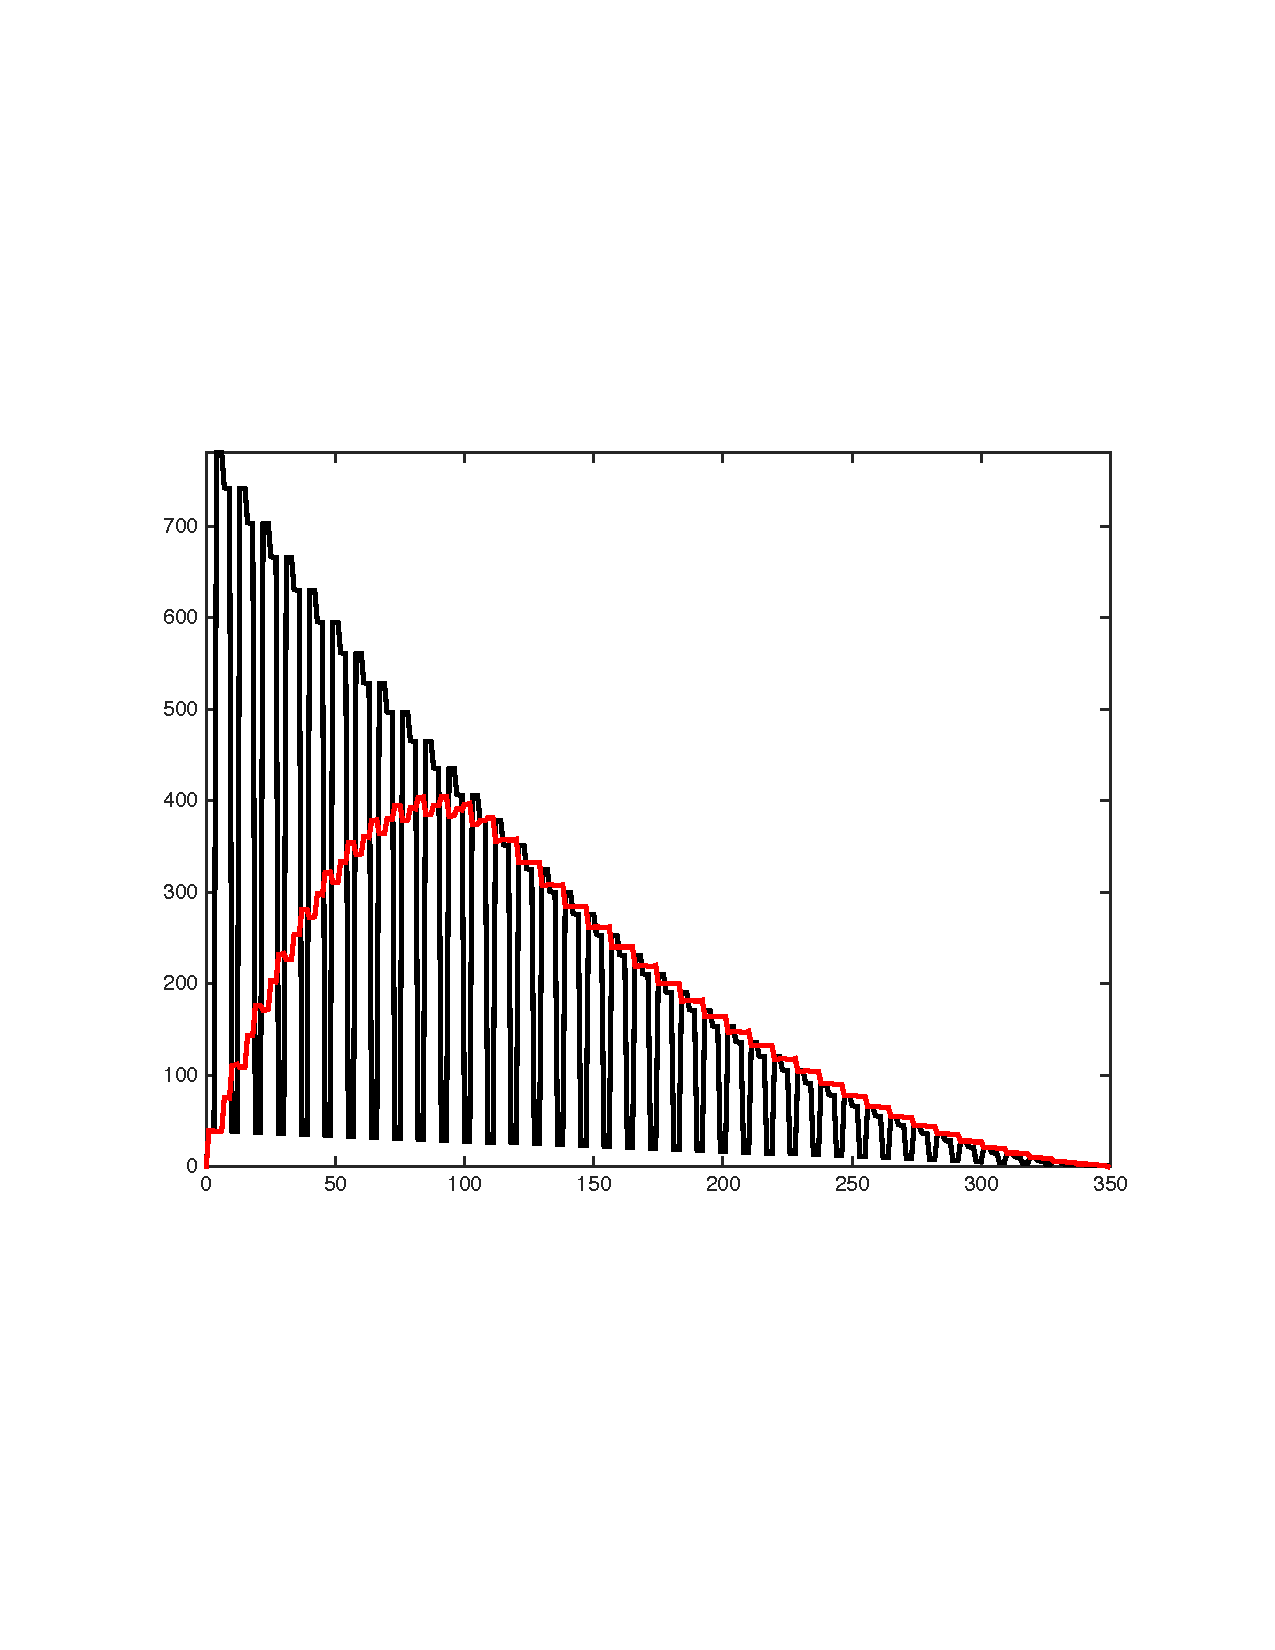
\includegraphics[width=.70\textwidth]{matlab_files/compare_ALAP_ASAP.pdf}\\
\scriptsize
$t=40$, \\
critical path length = $350$ ($= 9t-10$),\\
height of ALAP = 404 ($\approx \frac{1}{4}t^2 +\frac{1}{8}t$),\\
height of ASAP = 780 ($\approx \frac{1}{2}t^2 -\frac{1}{2}t$),\\
surface = $64,000$ ($=t^3$).


\end{frame}

\section{Using the ASAP and ALAP ``DAG'' to get new theoretical results}



\begin{frame}

Given a $t$-by-$t$ matrix with $t\geq2$,
we can guarantee that there exists a schedule which completes in $9t-10$
using $p_{CP,ALAP}(t)$ processors where $p_{CP,ALAP}(t)$ is given by

$$
p_{CP,ALAP}(t) = 
\frac{1}{4}t^2 +\frac{1}{8}t
 +\frac{1}{8}mod(t,8) + \frac{1}{2} mod( \lceil \frac{1}{2} mod(t,8) \rceil ,2)-1
$$

To simplify we can bound $p_{CP,ALAP}(t)$ below and above as
$$
\frac{1}{4}t^2 +\frac{1}{8}t -1
\leq  p_{CP,ALAP}(t) \leq 
\frac{1}{4}t^2 +\frac{1}{8}t + \frac{1}{4}.
$$



\end{frame}



\begin{frame}

We have that
$$ p_{CP,ALAP}(t) \approx \frac{1}{4}t^2 +\frac{1}{8}t .$$
How good is this?

We can compare with ASAP. For ASAP, we get
$$ p_{CP,ASAP}(t) = \frac{1}{2}t^2 -\frac{1}{2}t .$$

So ALAP completes in same time as ASAP but using about half the number of processors.


\end{frame}



\begin{frame}

We have that
$$ p_{CP,ALAP}(t) \approx \frac{1}{4}t^2 +\frac{1}{8}t .$$
How good is this?

We can also try to compare with any possible schedule.

Let $p_{CP,opt}(t)$ be the minimal number of processors to obtain the critical path.

Since we need to execute $t^3$ work and we want to complete in $9t-10$ time, we get
$$ p_{CP,opt}(t) \geq \frac{t^3}{9t-10}$$
so we get
$$ p_{CP,opt}(t) \geq \frac{1}{9}t^2+\frac{10}{81}t.$$

Can we get a better lower bound?



\end{frame}




\begin{frame}
\scriptsize

Given a fixed number of 
processing units, $p$, we give a lower bound on the execution time as follows:
$$\frac{t^{3}}{p} - 3\frac{t^2}{p} + 6\sqrt{2p} - 7.$$

We want to find the largest $p$ such that we can guarantee that any schedule will have an execution time greater than the critical path.

We want to find the largest $p$ such that
$$\frac{t^{3}}{p} - 3\frac{t^2}{p} + 6\sqrt{2p} - 7 \geq 9t - 10 $$
that is
$$ t^{3} - 3t^2 + 6\sqrt{2}p^{\frac{3}{2}}  \geq 9tp - 3p. $$

We set $p=\alpha t^2$.

We want to find the largest $\alpha$ such that
$$ t^{3} - 3t^2 + 6\sqrt{2}\alpha^{\frac{3}{2}} t^3  \geq 9\alpha t^3 - 3\alpha t^2 $$

Since $\alpha$ will be less than 1, we can remove the $t^2$ terms on both sides and get
that 
we want to find the largest $\alpha$ such that
$$ 1 + 6\sqrt{2}\alpha^{\frac{3}{2}}   \geq 9\alpha  $$
or 
$$  9\alpha  - 6\sqrt{2}\alpha^{\frac{3}{2}}  \geq 1 $$

We (numerically) find $\alpha < 0.187$.

Therefore we can say that any schedule which complete in $9t-10$ time needs at least 
$$ p_{CP,opt}(t) \geq 0.187 t^2.$$



\end{frame}




\begin{frame}

So we naievely get
$$ 0.111 t^2 \leq p_{CP,opt}(t) \leq 0.500 t^2 $$

And with our work, we get
$$ 0.187 t^2 \leq p_{CP,opt}(t) \leq 0.250 t^2 $$

\end{frame}




\begin{frame}

How to work a lower bound?\\

\begin{minipage}{5cm}
For $t=6$,\\
Time is at least $9t-10 = 44$.\\
Time is at least $t^3/p = 216/p$.\\ 
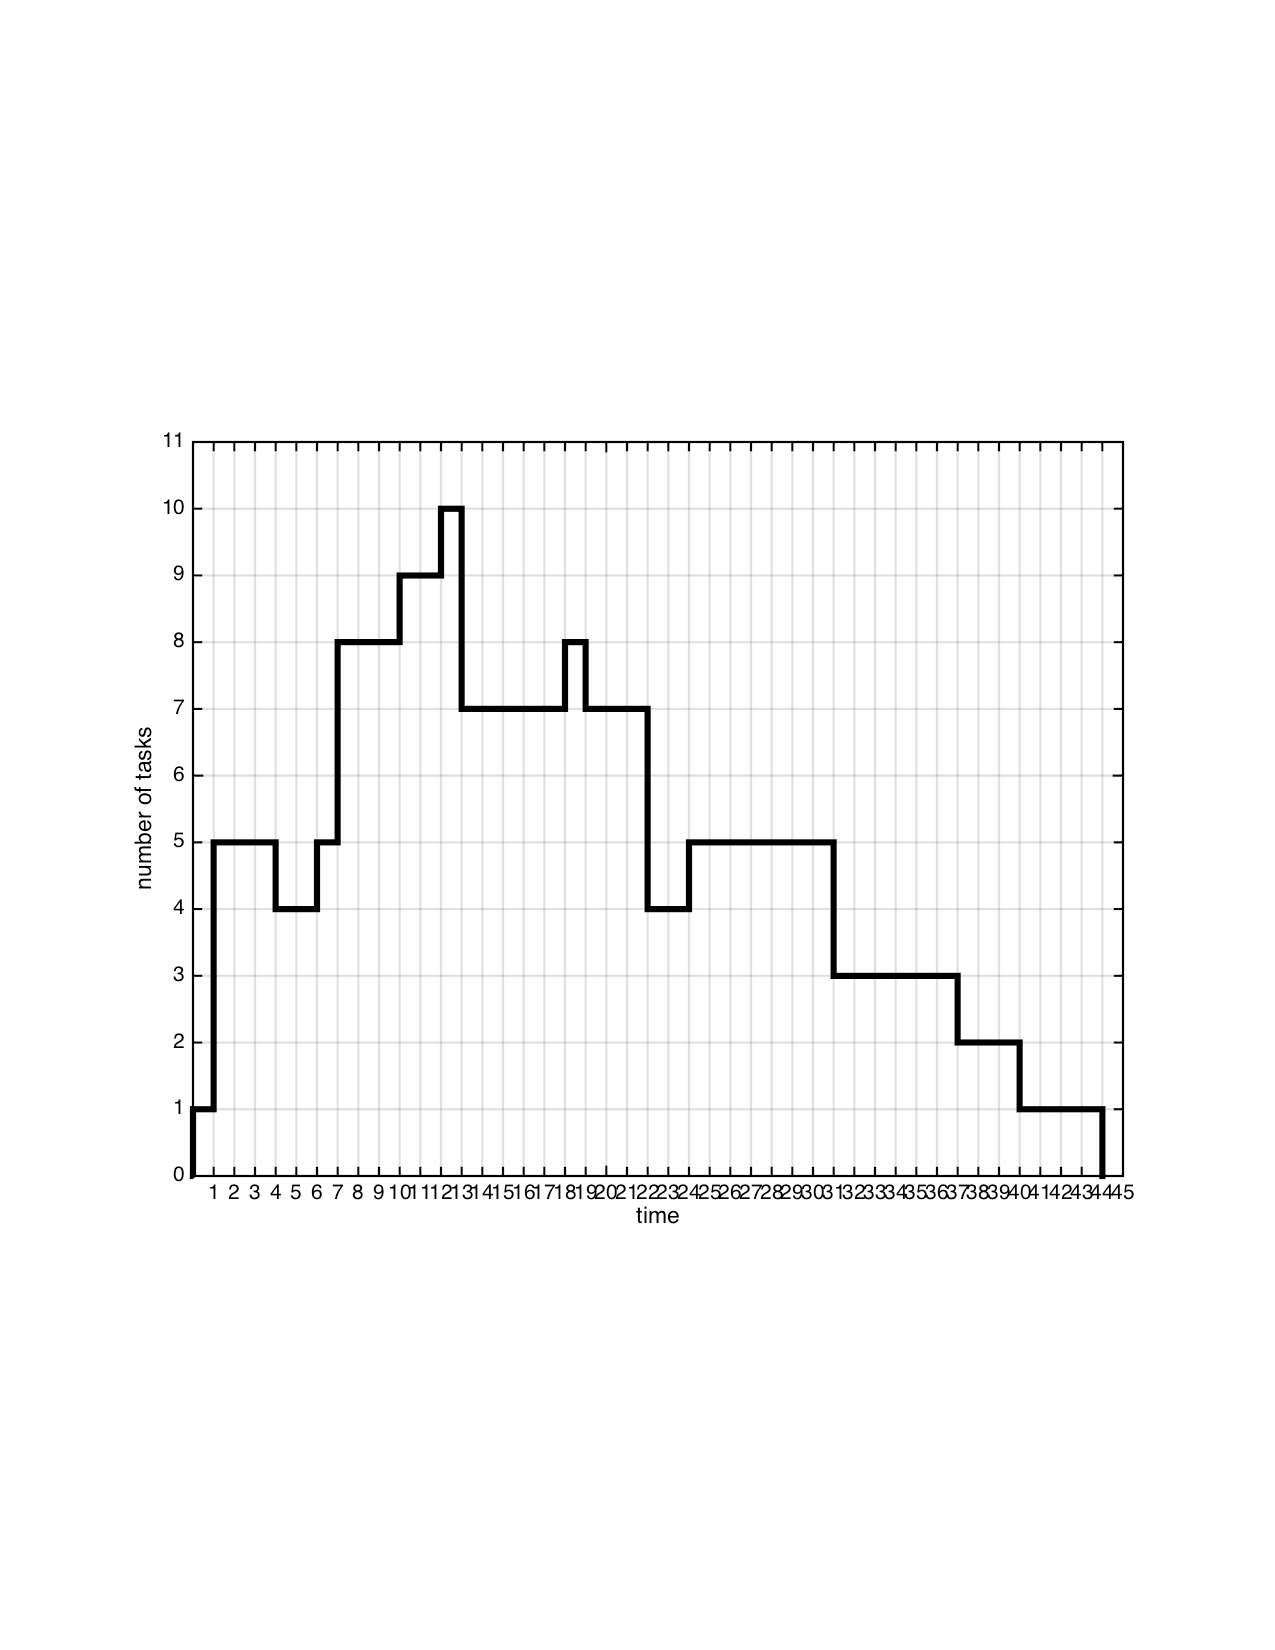
\includegraphics[width=\textwidth]{dague_faverge/qqq_t6.pdf}\\
\end{minipage}
\begin{minipage}{5cm}
For $p=2$, time is at least:
$$ (216 - 4 ) / 2 + 4 $$
For $p=3$, time is at least:
$$ (216 - 10 ) / 3 + 7 $$
For $p=4$, time is at least:
$$ (216 - 28 ) / 3 + 13 $$

For $p$, time is at least:
$$ 216/p - VOL_w(p) / p + CP_w(p) $$
\end{minipage}



\end{frame}



\begin{frame}





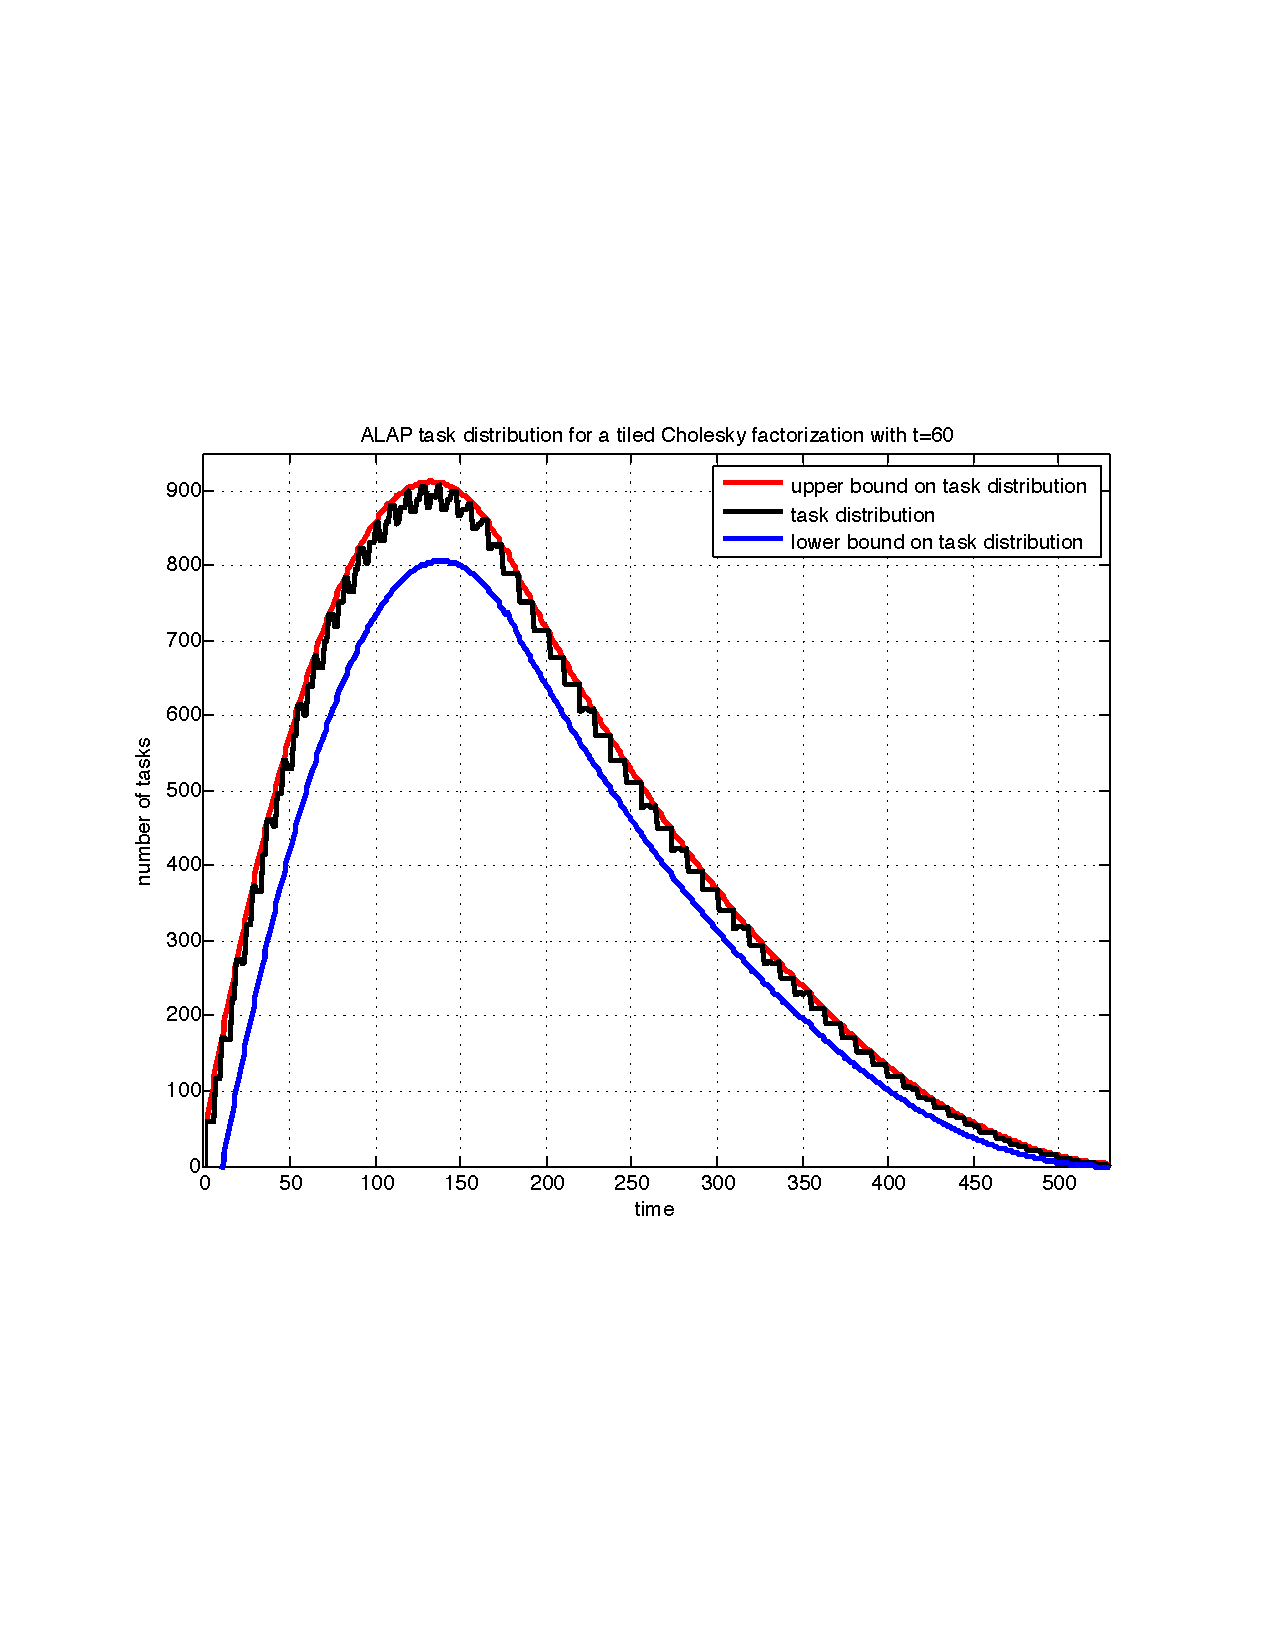
\includegraphics[width=3in]{matlab_files/bornesV2_60.pdf}\\
{\bf Figure.} ALAP distribution for $t=60$ tiles. In black is the exact distribution. Red is the upper bound. Blue is the lower bound.




\end{frame}



\begin{frame}





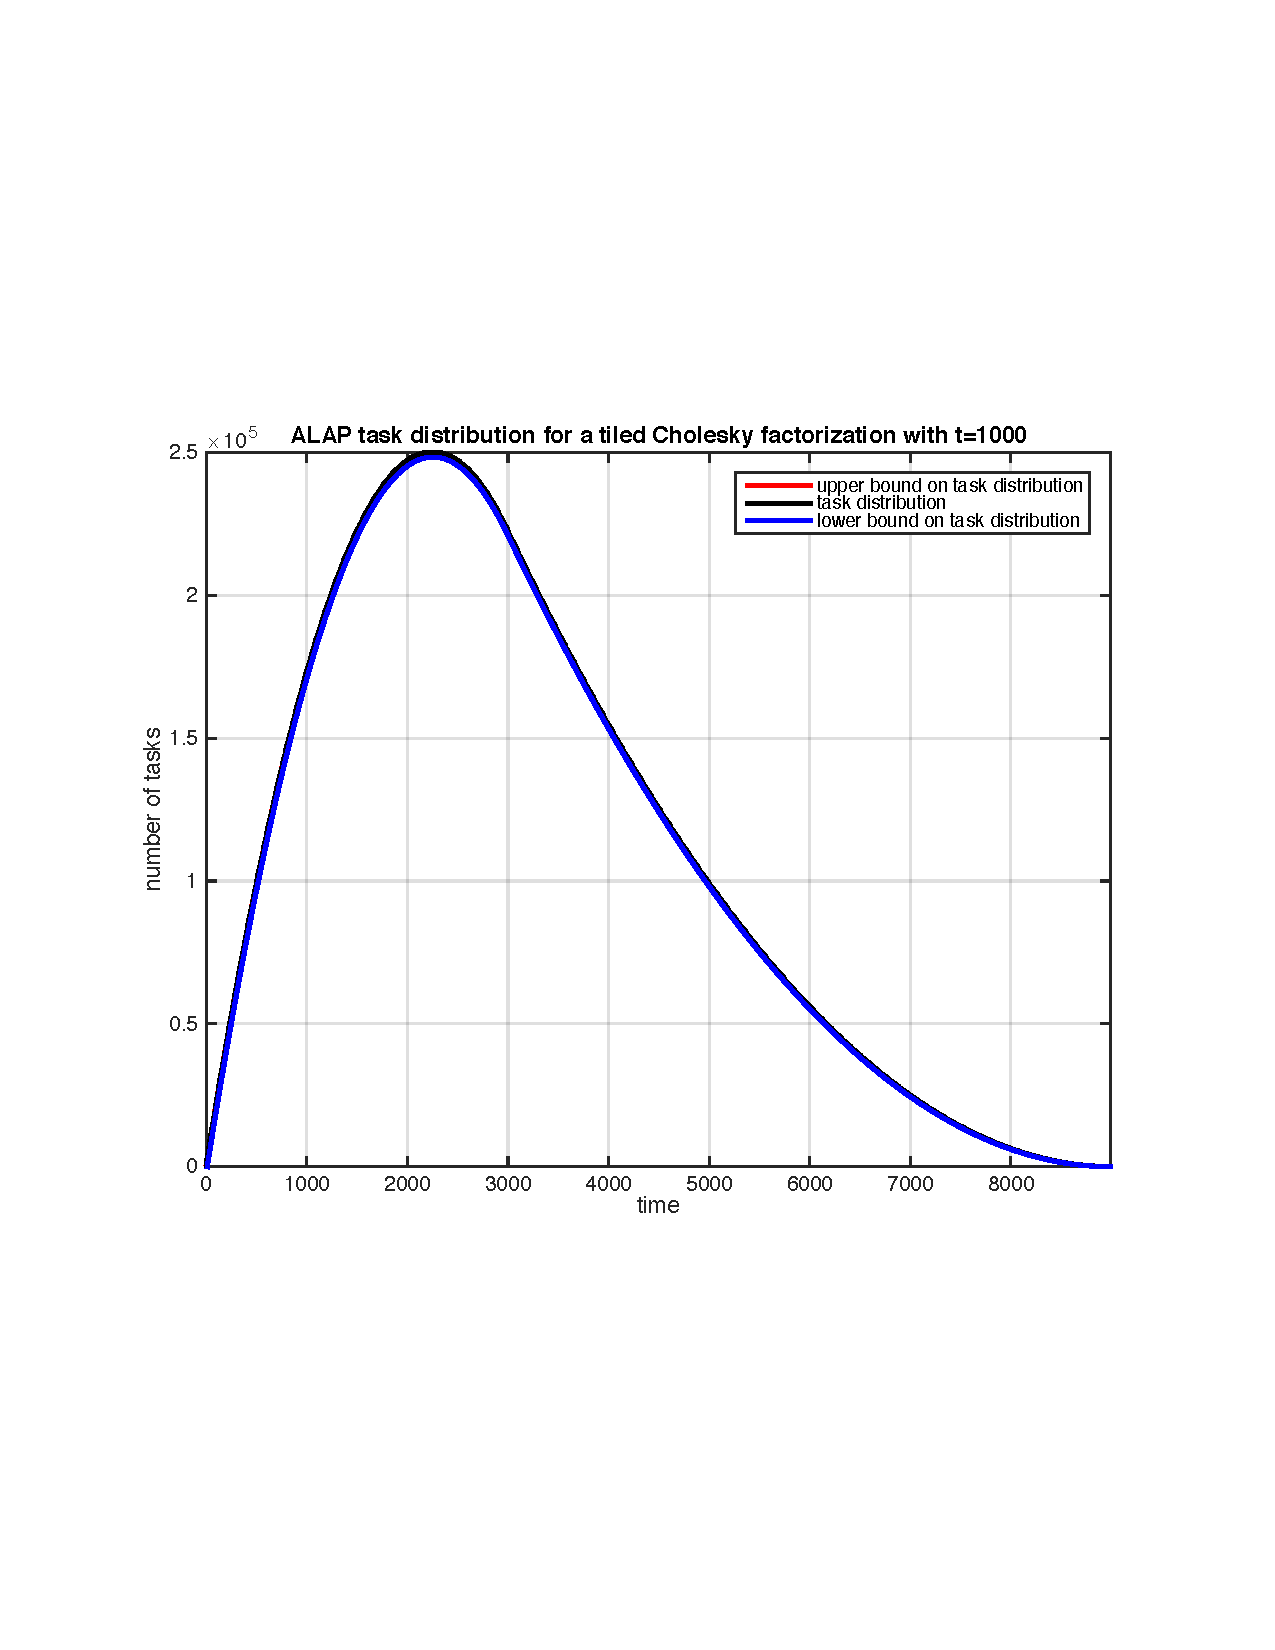
\includegraphics[width=3in]{matlab_files/bornesV2_1000.pdf}\\
{\bf Figure.} ALAP distribution for $t=1000$ tiles. In black is the exact distribution. Red is the upper bound. Blue is the lower bound.




\end{frame}











\begin{frame}


\begin{tabular}{|c|c|}
  \hline
  Zone & Lower bound on height \\
  \hline
  1  & $\frac{K^{2}}{162}-\frac{5K}{162}-\frac{25}{81}$\\
  \hline
  2  & $\frac{K^{2}}{162}-\frac{16K}{162}+\frac{t}{2}-\frac{289}{324}$\\
  \hline
  3  & $-\frac{4K^{2}}{81}+\frac{2Kt}{3}-\frac{197K}{162}-2t^{2}+\frac{119t}{18}-\frac{587}{108}$ \\
  \hline
\end{tabular}\\
{\bf Table.} Lower bound on the height of the ALAP schedule\\

\vspace*{1cm}
\noindent
\begin{tabular}{|c|c|}
  \hline
  Zone & Upper bound on height \\
  \hline
  1  & $\frac{K^{2}}{162}+\frac{31K}{162}+\frac{155}{81}$\\
  \hline
  2  & $\frac{K^{2}}{162}+\frac{2K}{81}+\frac{t}{2}+\frac{755}{324} $\\
  \hline
  3  & $-\frac{4K^{2}}{81}+\frac{2Kt}{3}-\frac{107K}{162}-2t^{2}+\frac{83t}{18}+\frac{37}{108}$ \\
  \hline
\end{tabular}\\
{\bf Table.} 
Upper bound on the height of the ALAP schedule



\end{frame}



\begin{frame}






\begin{block}{Lower bound on the makespan of the Cholesky factorization}
Any schedule working with $p$ processing units on the $t\times t$ tiled Cholesky factorization has an execution time greater than:
$$\max( \frac{t^{3}}{p}, 
\frac{t^{3}}{p} - 3\frac{t^2}{p} + 6\sqrt{2p} - 7 ,
9t-10).$$
\end{block}




\end{frame}


\section{Applications to scheduling}


\begin{frame}

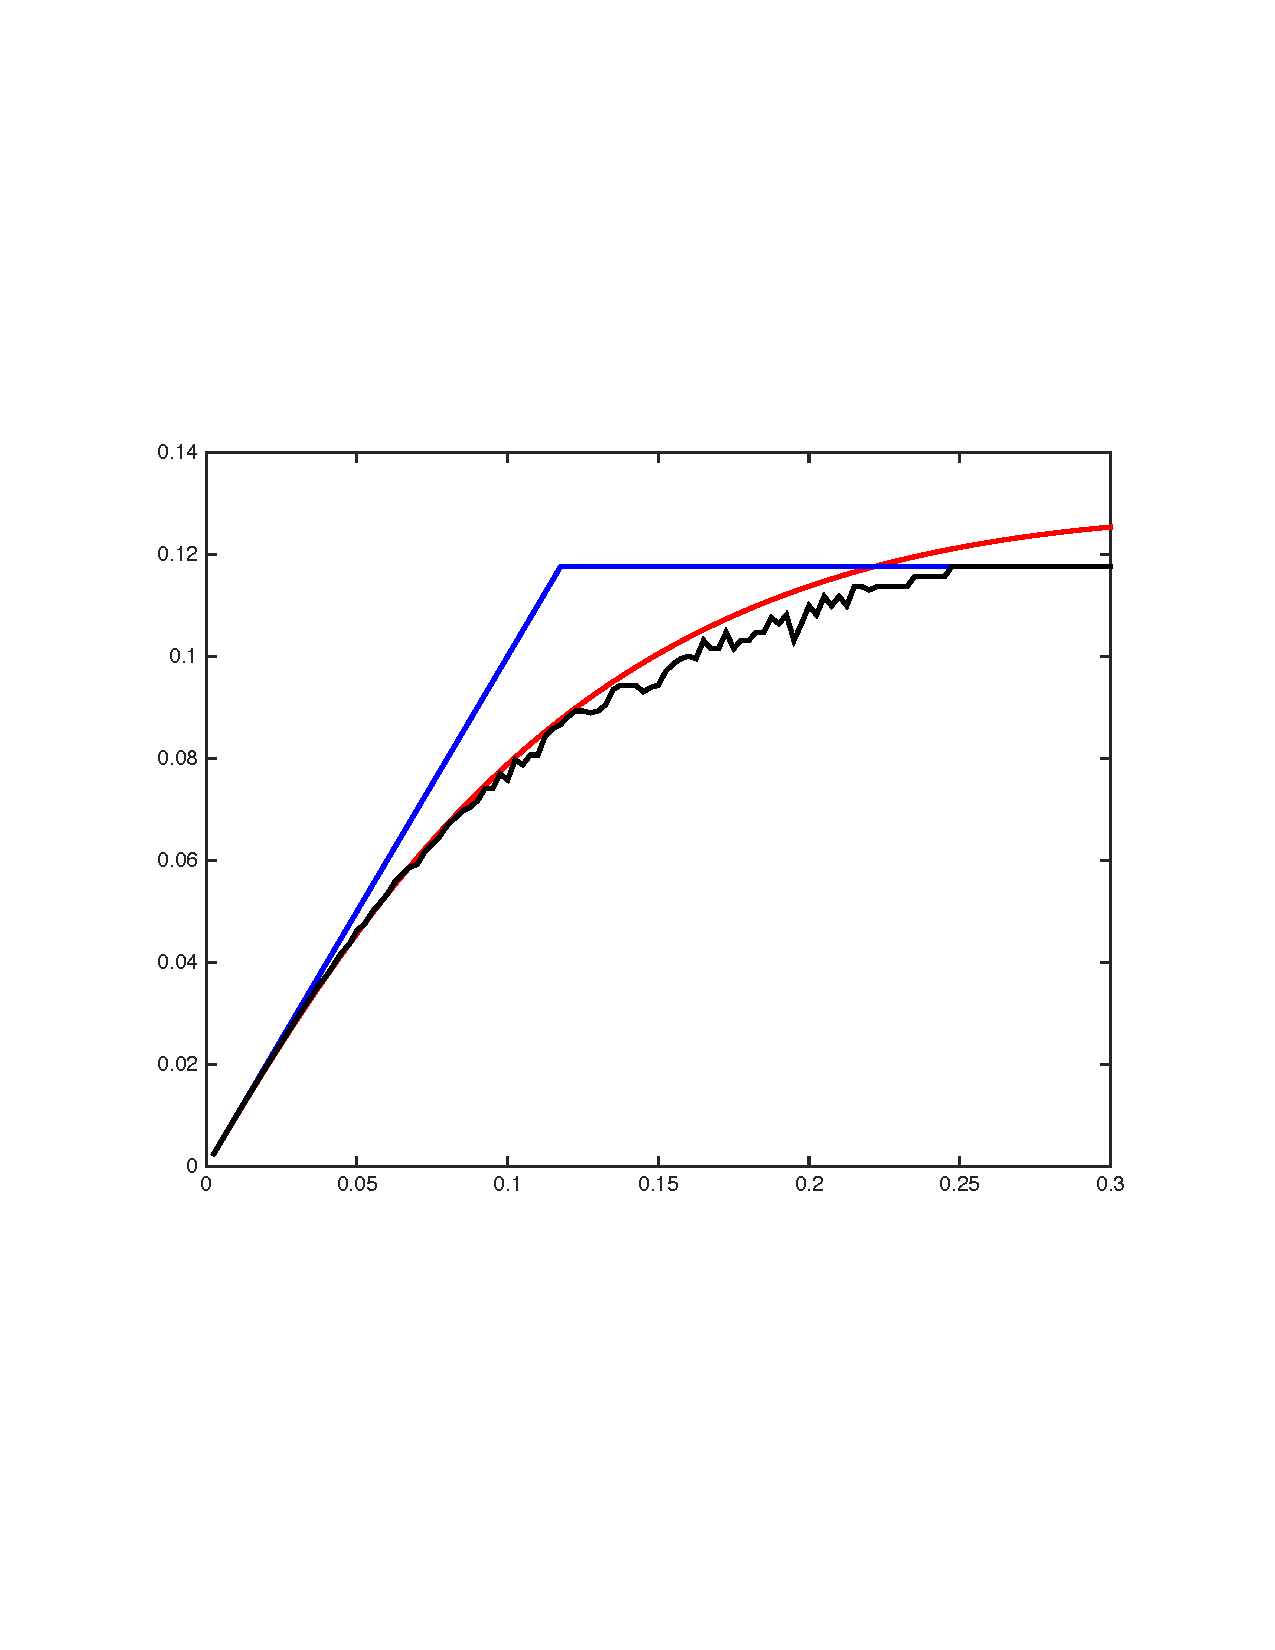
\includegraphics[width=.80\textwidth]{matlab_files/CheckWithSomeScheduling_t20.pdf}\\

\end{frame}



\begin{frame}

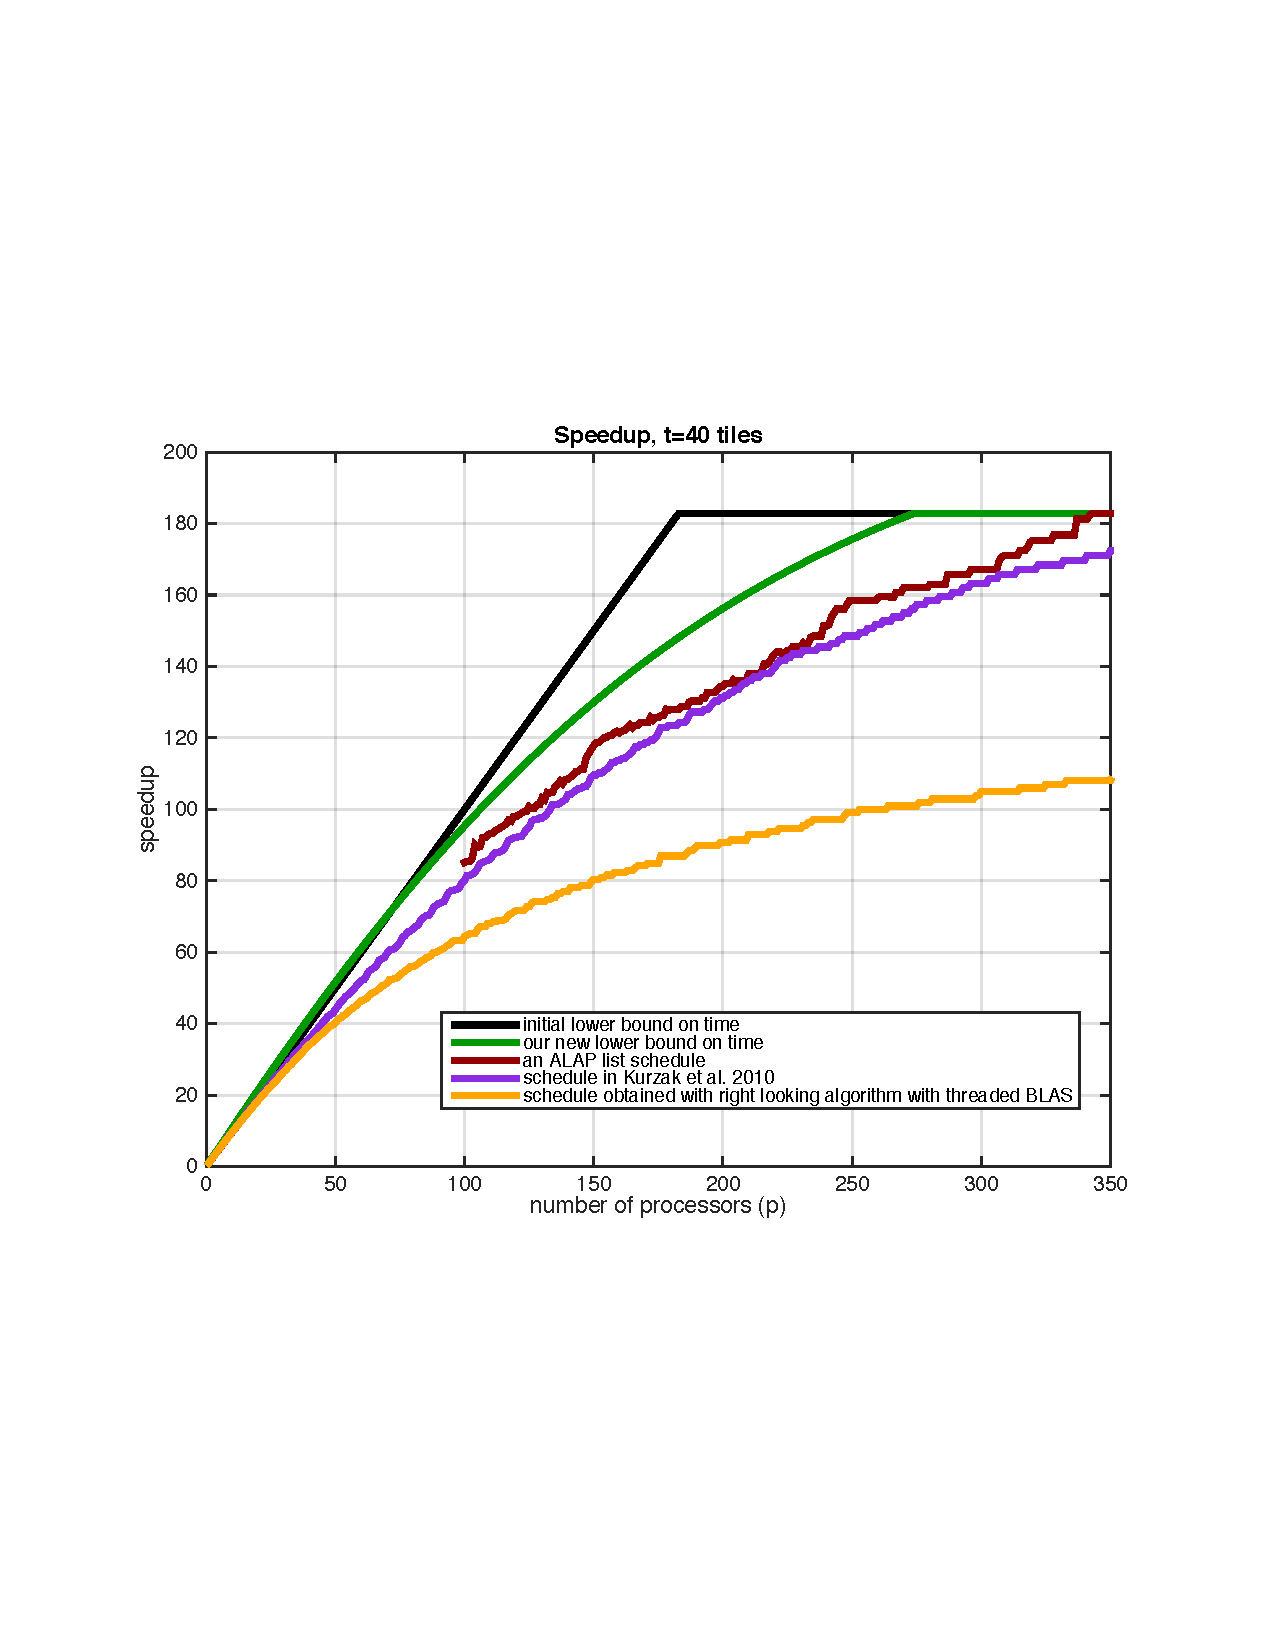
\includegraphics[width=.80\textwidth]{matlab_files/borneTempsExecByProc_CLEANED_fig1.pdf}\\

\end{frame}



\begin{frame}

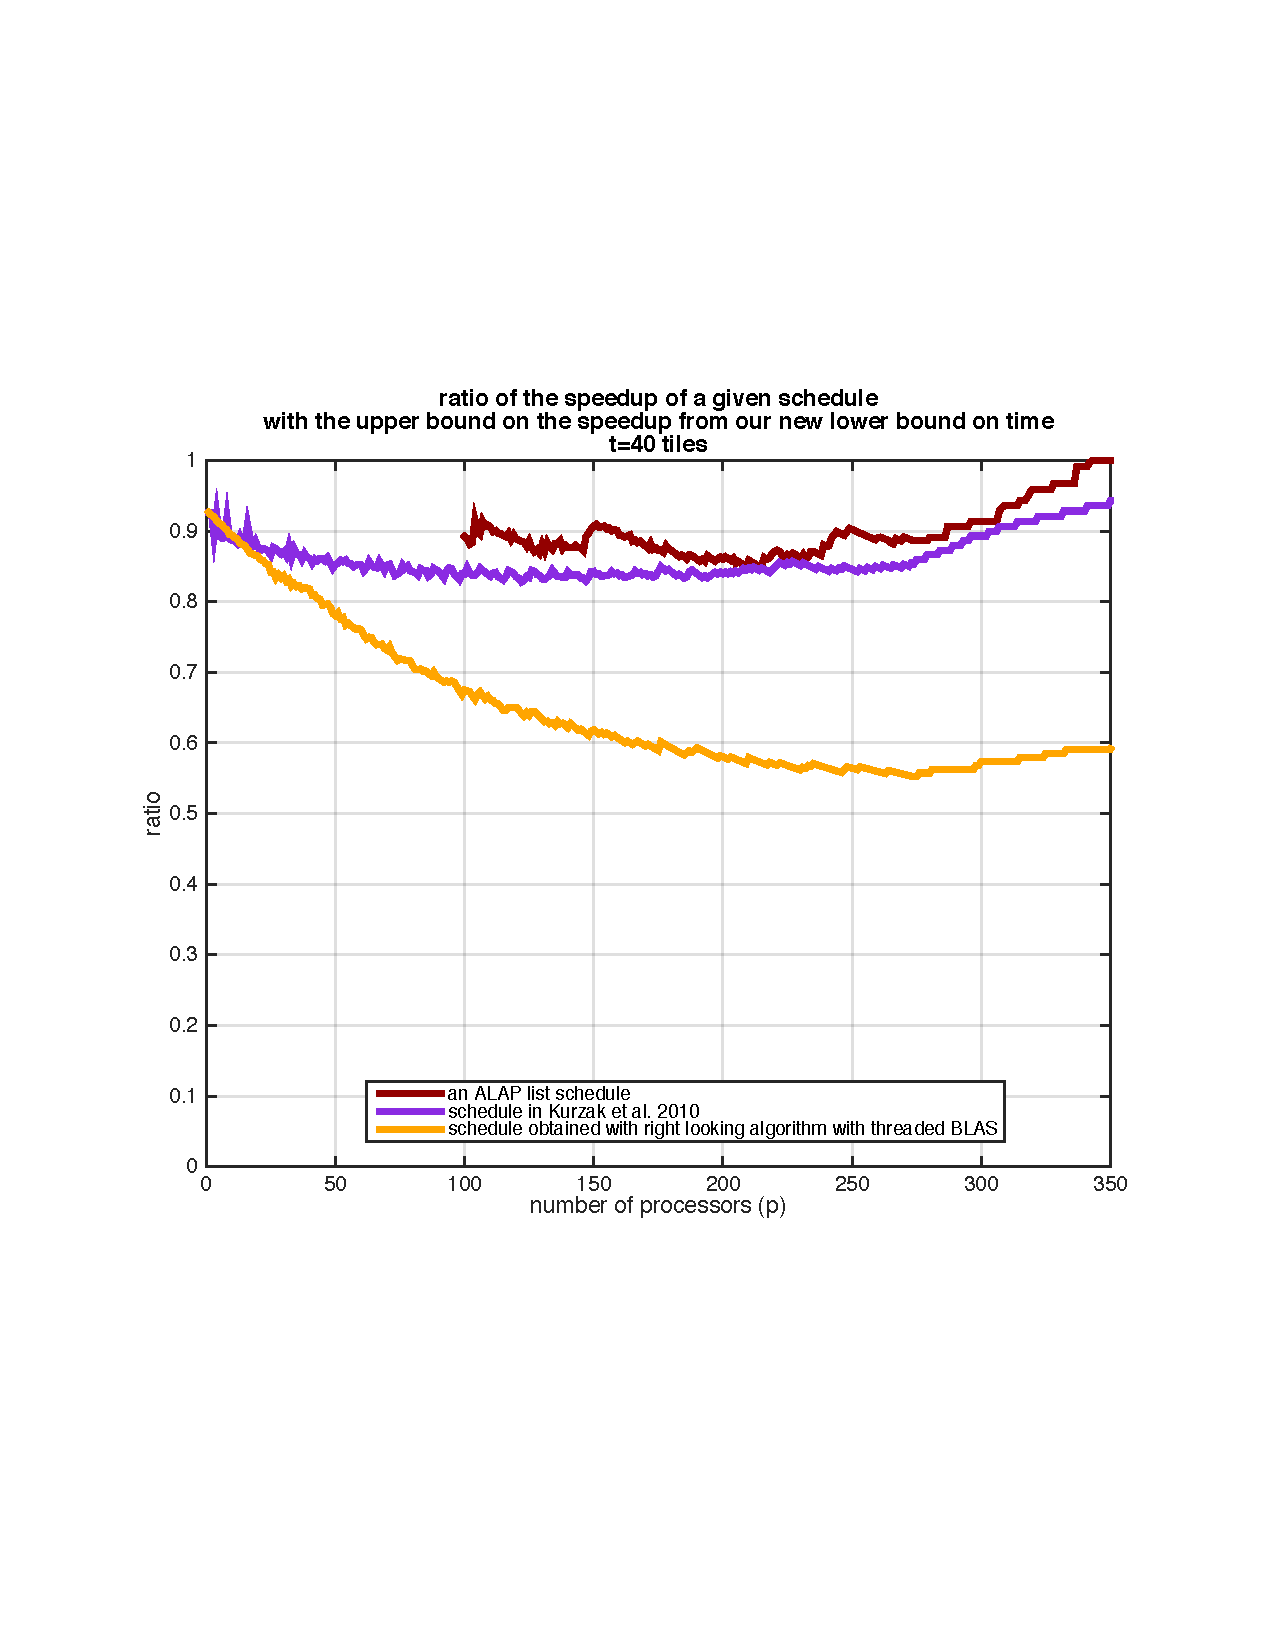
\includegraphics[width=.80\textwidth]{matlab_files/borneTempsExecByProc_CLEANED_fig3.pdf}\\

\end{frame}

\section{Applications to DPLASMA}

\begin{frame}

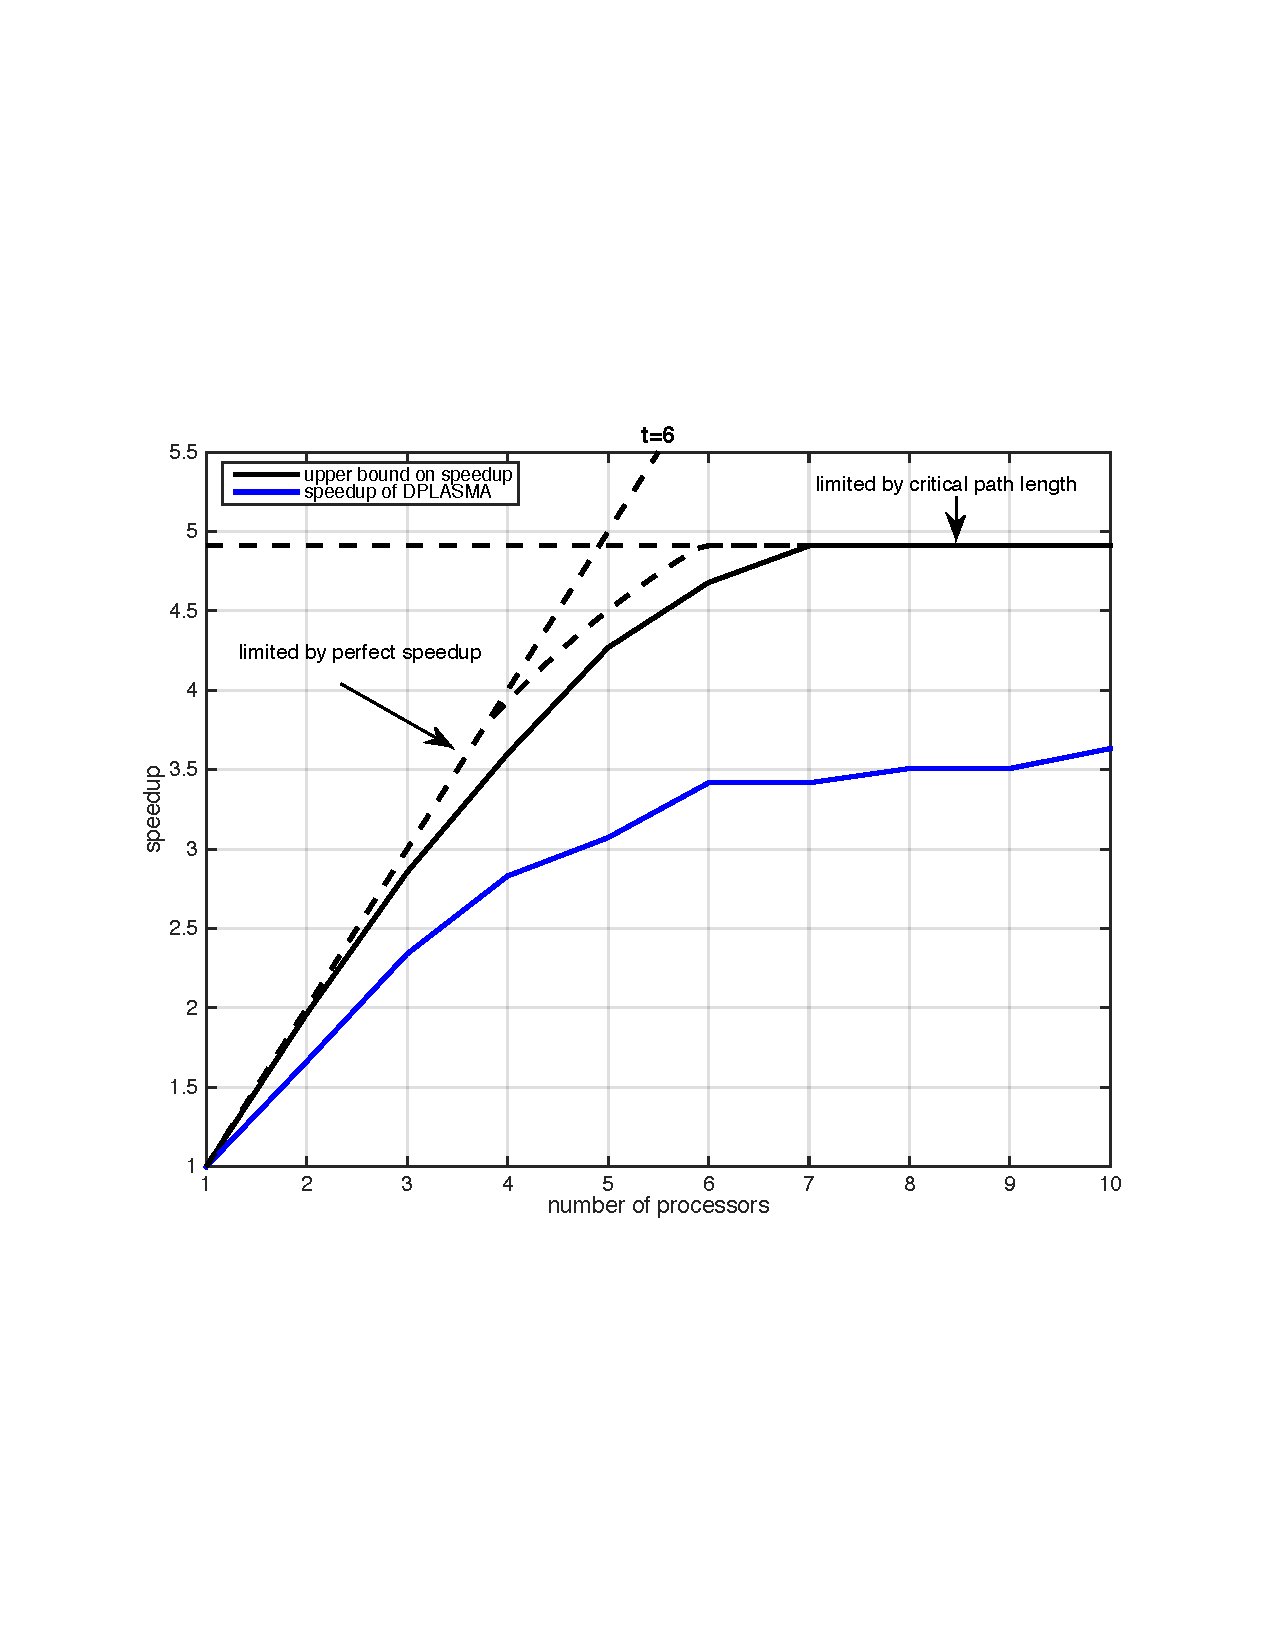
\includegraphics[width=.80\textwidth]{dague_faverge/plot__t6.pdf}\\

This is a shared memory experiment. Block size is 200.


\end{frame}


\begin{frame}

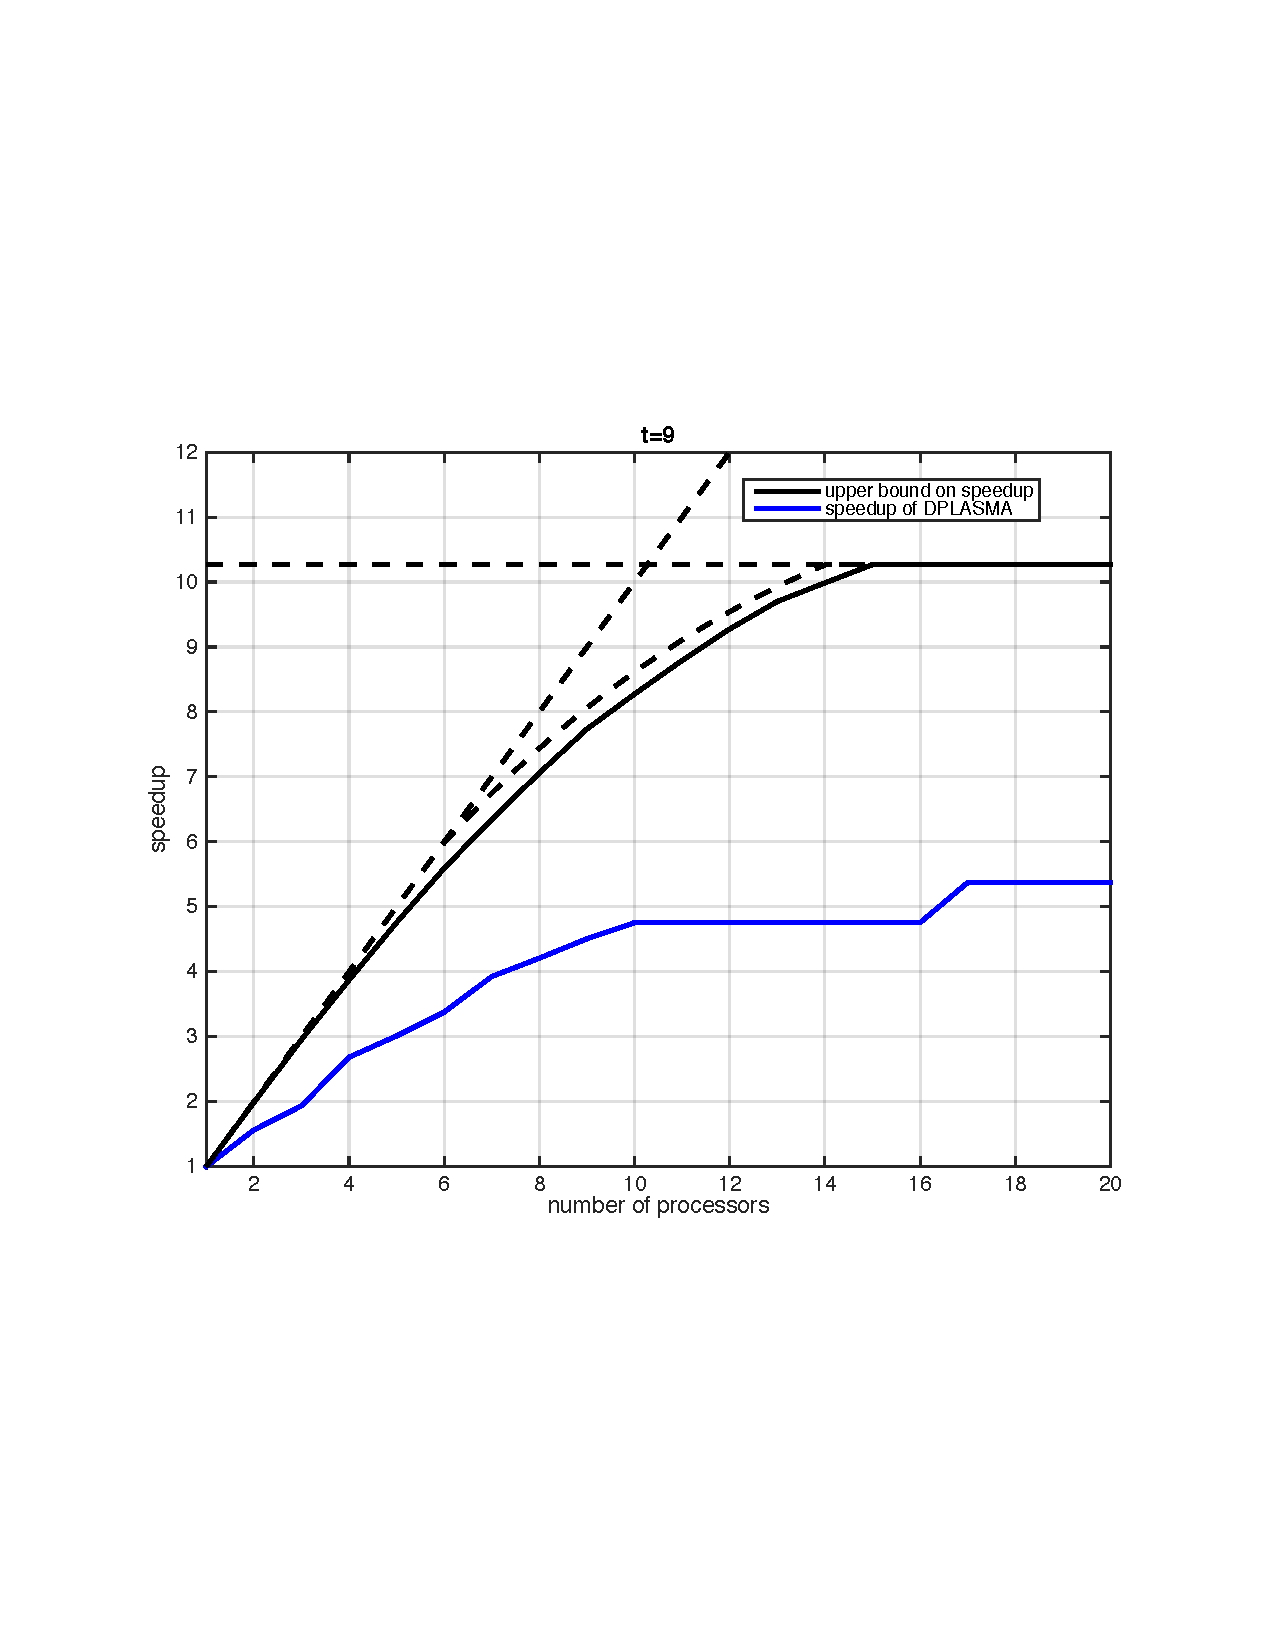
\includegraphics[width=.80\textwidth]{dague_faverge/plot__t9.pdf}\\

This is a shared memory experiment. Block size is 200.

\end{frame}



\begin{frame}

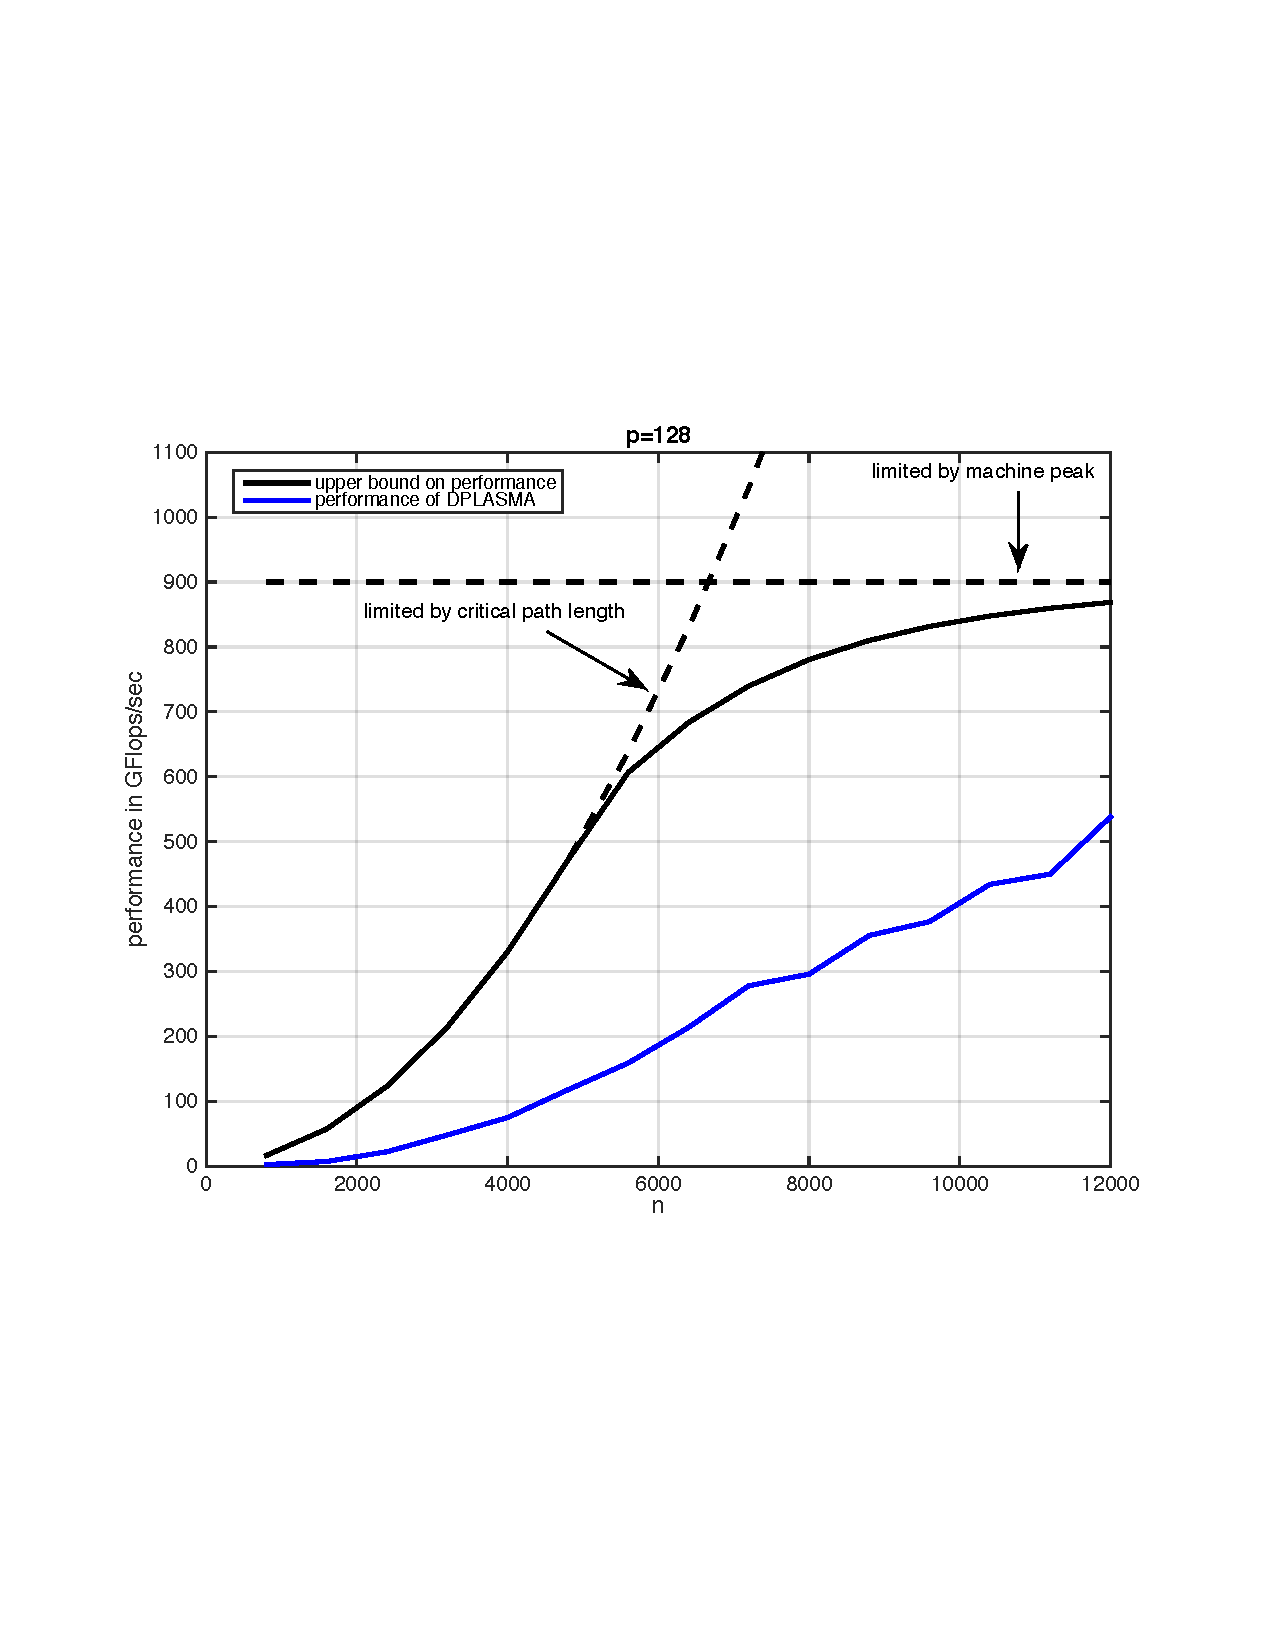
\includegraphics[width=.80\textwidth]{dague_faverge/data3.pdf}\\
block size is 200, we use 16 nodes in a 4x4 grid, 8 cores per node\\
$p$ is fixed at 128\\
$n$ ranges from 800 to 12,000, so $t$ ranges from 4 to 20.


\end{frame}


\section{}

 \begin{frame}
   \tableofcontents
 \end{frame}


\begin{frame}

\footnotesize
\nocite{konig1988}
%\nocite{konig:hal-00857003}
\nocite{COSNARD1988275}
%\nocite{cosnard:hal-00857005}
\nocite{j38}
\nocite{Robert1989159}
%\nocite{journals/pc/MarrakchiR89}
\nocite{Kurzak2008}


\bibliographystyle{IEEEtran}


  \bibliography{../biblio/biblio}



\end{frame}






\begin{frame}

Comment \#1
\begin{itemize}
\item ALAP seems better suited than ASAP for linear algebra
\item Exploits this fact for lower bound and schedule
\end{itemize}

\vspace*{1cm}

Comment \#2
\begin{itemize}
\item Our formulae are geared toward an assymptotic analysis.
\item Some formulae are exact. In which case, great.
\item Our formulae are not very good for small $t$ and $p$. For small $t$ and $p$, we can use matlab code for analysis and get tighter bounds
\end{itemize}

\end{frame}






\begin{frame}

What is next?
\begin{itemize}
\item Derive better schedule through ALAP, study more schedule, 
\begin{itemize}
\item How do you schedule backward?
\end{itemize}
\item Find other techniques than ALAP for lower bounds
\begin{itemize}
\item Refine the techniques
\end{itemize}
\item Use these ``better'' schedules in practice for demo runs (DPLASMA?)
\item Automate all this (compilers?)
\begin{itemize}
\item Would be able use any weights, any DAG, more precise than formulae
\end{itemize}
\item Extend to other linear algebra operations
\item Take data distribution and communication into account
\item Direct impact on energy (idle+work) bounds,
\begin{itemize}
\item Multi-criteria optimization with time to solution
\end{itemize}
\item Publish work (!)
\end{itemize}

See:
http://arxiv.org/abs/1510.05107

\end{frame}




\begin{frame}

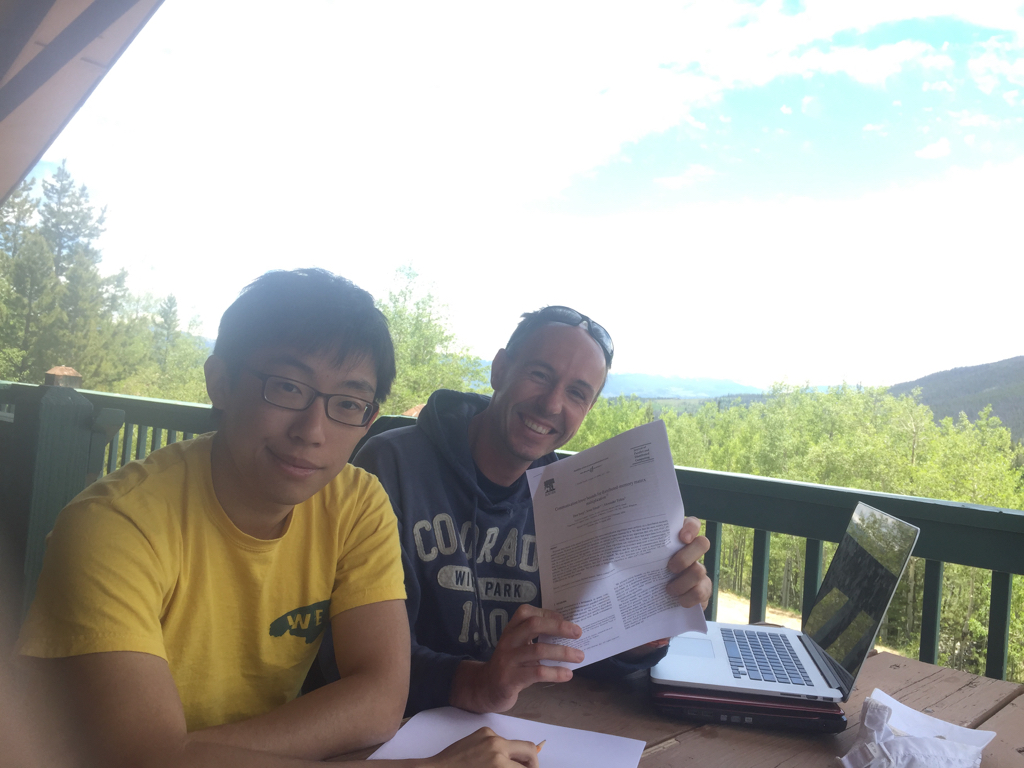
\includegraphics[width=.50\textwidth]{willy.jpg}\\

\end{frame}






\end{document} 

